\chapter[Συστηματα]{Συστηματα} 
\section{Γραμμικά Συστήματα}
\orismoi
\begin{orismos}{Γραμμική Εξίσωση}
Γραμμική εξίσωση δύο μεταβλητών, ονομάζεται κάθε εξίσωση της μορφής \[ ax+\beta y=\gamma \]
\end{orismos}
\begin{itemize}[itemsep=0mm]
\item Οι μεταβλητές της εξίσωσης είναι οι $ x,y $.
\item Οι πραγματικοί αριθμοί $ a,\beta\in\mathbb{R} $ λέγονται \textbf{συντελεστές} των μεταβλητών.
\item Ο πραγματικός αριθμός $ \gamma\in\mathbb{R} $ ονομάζεται \textbf{σταθερός όρος} της εξίσωσης.
\end{itemize}
Εν παραδείγματι μια γραμμική εξίσωση με μεταβλητές $ x,y $, είναι η $ 2x+y=5 $. Στη γραμμική εξίσωση αυτή, συντελεστές των μεταβλητών $ x,y $ είναι αντίστοιχα οι $ 2 $ και $ 1 $, ενώ σταθερός όρος της είναι το $ 5 $. Χρειάζονται $ 2 $ αριθμοί προκειμένου να επαληθευτεί μια τέτοια εξίσωση οι οποίοι θα σχηματίσουν τη λύση αυτής που ορίζεται ως εξής:
\begin{orismos}{Λύση γραμμικής εξίσωσης}
Λύση μιας γραμμικής εξίσωσης της μορφής \[ ax+\beta y=\gamma \] ονομάζεται κάθε διατεταγμένο ζεύγος αριθμών $ \left( x_0,y_0\right)  $ το οποίο επαληθεύει την εξίσωση.
\end{orismos}
Παρατηρούμε εύκολα ότι οι αριθμοί $ x=2$ και  $y=1 $ επαληθεύουν την εξίσωση που αναφέραμε στο παράδειγμα αφού αντικαθιστώντας παίρνουμε
\[ 2x+y=5\Rightarrow 2\cdot 2+1=5\Rightarrow 5=5 \] άρα το ζεύγος $ (x,y)=(2,1) $ αποτελεί λύση της εξίσωσης. Όπως θα δούμε στις ασκήσεις παρακάτω, το ζεύγος αυτό δεν είναι μοναδικό. Μια γραμμική εξίσωση $ 2 $ μεταβλητών έχει άπειρες λύσεις, όπου αυτές έχουν συγκεκριμένη μορφή την οποία και θα αναζητήσουμε.
\begin{orismos}{Γραμμικό σύστημα $ \mathbold{2\times2} $}
Γραμμικό σύστημα δύο εξισώσεων με δύο άγνωστους ονομάζεται ο συνδυασμός - σύζευξη δύο γραμμικών εξισώσεων. Είναι της μορφής :
\begin{equation}\label{systhma}
\ccases{{a}x+{\beta} y={\gamma}\\{a'}x+{\beta'} y={\gamma'} }
\end{equation}
\end{orismos}
\begin{itemize}[itemsep=0mm]
\item Οι αριθμοί $ a,a',\beta,\beta'\in\mathbb{R} $ ονομάζονται \textbf{συντελεστές} του συστήματος ενώ οι $ \gamma,\gamma'\in\mathbb{R} $ λέγονται \textbf{σταθεροί όροι}.
\item Κάθε διατεταγμένο ζεύγος αριθμών $ \left(x_0,y_0\right)  $ το οποίο επαληθεύει και τις δύο εξισώσεις ονομάζεται \textbf{λύση} του γραμμικού συστήματος.
\item Τα συστήματα τα οποία έχουν ακριβώς τις ίδιες λύσεις ονομάζονται \textbf{ισοδύναμα}.
\item Ένα σύστημα που έχει λύση λέγεται \textbf{συμβιβαστό}. Εάν δεν έχει λύση ονομάζεται \textbf{αδύνατο} ενώ αν έχει άπειρες λύσεις \textbf{αόριστο}.
\item Η διαδικασία με την οποία ελέγχουμε αν ένα ζεύγος αριθμών αποτελεί λύση ονομάζεται \textbf{επαλήθευση} του συστήματος.
\end{itemize}
Συνδυάζοντας την εξίσωση του παραδείγματος με την $ x-3y=-1 $ παίρνουμε το γραμμικό σύστημα
\begin{equation}\label{grsys:systhma}
\systeme{2x+y=5,x-3y=-1}
\end{equation}
το οποίο είναι συμβιβαστό καθώς έχει μοναδική λύση το ζευγάρι $ (x,y)=(2,1) $. Στο σύστημα αυτό, συντελεστές της μεταβλητής $ x $ είναι οι $ 2 $ και $ 1 $, η μεταβλητή $ y $ έχει συντελεστές τους $ 1 $ και $ -3 $ και σταθεροί όροι του συστήματος είναι οι $ 5 $ και $ -1 $. Εύκολα διαπιστώνουμε με αντικατάσταση ότι το ζεύγος $ (x,y)=(2,1) $ είναι λύση του συστήματος \eqref{grsys:systhma} ως εξής: Για $ x=2 $ και $ y=1 $
\[ \ccases{2\cdot 2+1=5\\2-3\cdot 1=-1}\Rightarrow \ccases{5=5\\-1=-1} \]
άρα επαληθεύονται και οι δύο εξισώσεις.
\begin{orismos}{Ορίζουσα Συστήματος {$ \mathbold{2\mathbold{\times}2} $}}
Θεωρούμε ένα γραμμικό σύστημα $ 2\times2 $ της μορφής \eqref{systhma}. Ορίζουσα των συντελεστών ονομάζεται ο αριθμός $ a\beta'-a'\beta $ και συμβολίζεται με $ D $. Μπορεί να γραφτεί στη μορφή πίνακα όπως φαίνεται παρακάτω:
\[ D=\left|\begin{array}{cc}
a & \beta \\ 
a' & \beta'
\end{array}  \right|  \]
Επίσης $ D_x,D_y $ είναι οι ορίζουσες των μεταβλητών που προκύπτουν αν αντικαταστήσουμε στην ορίζουσα $ D $ τη στήλη των συντελεστών των μεταβλητών $ x,y $ αντίστοιχα με τους σταθερούς όρους $ \gamma,\gamma' $. Θα είναι:
\[ D_x=\left|\begin{array}{cc}
\gamma & \beta \\ 
\gamma' & \beta'
\end{array}  \right|=\gamma\beta'-\gamma'\beta\quad,\quad D_y=\left|\begin{array}{cc}
a & \gamma \\ 
a' & \gamma'
\end{array}  \right|=a\gamma'-a'\gamma \]
\end{orismos}
Ο υπολογισμός μιας $ 2\times 2 $ ορίζουσας γίνεται πολλαπλασιάζοντας τους αριθμούς των δύο στηλών "χιαστί" όπως μας δείχνει το παρακάτω διάγραμμα. Παρατηρούμε ότι παίζει ρόλο η σειρά με την οποία αφαιρούνται τα δύο γινόμενα.
\begin{center}
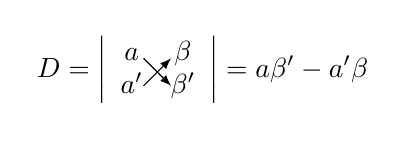
\begin{tikzpicture}
\node at (0,0){$ D=\left|\begin{array}{cc}
a & \beta \\ 
a' & \beta'
\end{array}  \right|=a\beta'-a'\beta $};
\draw[-latex] (-.75,.15)--(-.4,-0.2);
\draw[-latex] (-.75,-0.2)--(-.4,.15);
\end{tikzpicture}
\end{center}
Το γραμμικό σύστημα \[ \systeme{2x+y=5,x-3y=-1} \] που είδαμε παραπάνω έχει τις εξής ορίζουσες. Ορίζουσα των συντελεστών είναι η 
\[ D=\begin{vmatrix}
2 & 1\\ 1 & -3
\end{vmatrix}=2\cdot(-3)-1\cdot1=-7 \]
Ομοίως οι ορίζουσες των μεταβλητών $ x,y $ θα είναι αντίστοιχα
\[ D_x=\begin{vmatrix}
5 & 1\\-1 & -3
\end{vmatrix}=5\cdot(-3)-1\cdot(-1)=-14\ \ \textrm{και} \]
\[ D_y=\begin{vmatrix}
2 & 5\\ 1 & -1
\end{vmatrix}=2\cdot(-1)-5\cdot 1=-7 \]
\begin{orismos}{Γραμμικό Σύστημα Εξισώσεων $ \mathbold{3\times3} $}
Γραμμικό σύστημα τριών εξισώσεων με τρεις άγνωστους ονομάζεται ένας συνδυασμός από τρεις γραμμικές εξισώσεις της μορφής
\[ \ccases{{a_1}x+{\beta_1} y+{\gamma_1} z=\delta_1\\{a_2}x+{\beta_2} y+{\gamma_2} z=\delta_2\\{a_3}x+{\beta_3} y+{\gamma_3} z=\delta_3} \]
με $ a_i,\beta_i,\gamma_i,\delta_i\in\mathbb{R}\;,\;i=1,2,3 $. Κάθε διατεταγμένη τριάδα αριθμών $ \left( x_0,y_0,z_0\right)  $ η οποία επαληθεύει και τις τρεις εξισώσεις ονομάζεται \textbf{λύση} του γραμμικού συστήματος $ 3\times3 $.
\end{orismos}
Το ακόλουθο $ 3\times3 $ γραμμικό σύστημα με μεταβλητές $ x,y $ και $ z $
\[ \csysteme{x-2y+z=3,3x-y+4z=16,-2x+3y-z=-5} \]
έχει ως λύση τη διατεταγμένη τριάδα $ (x,y,z)=(3,1,2) $. το οποίο επαληθεύεται εύκολα με αντικατάσταση.
\begin{orismos}{Παραμετρικό σύστημα}
Παραμετρικό ονομάζεται το γραμμικό σύστημα του οποίου οι συντελεστές ή και οι σταθεροί όροι δίνονται με τη βοήθεια μιας ή περισσότερων παραμέτρων. Η διαδικασία επίλυσης ενός παραμετρικού συστήματος ονομάζεται \textbf{διερεύνηση}.
\end{orismos}
Το παρακάτω παραμετρικό γραμμικό σύστημα
\[ \systeme{{(\lambda+1)}x+y=2,2x+\lambda y=\lambda+1} \]
για τις διάφορες τιμές της παραμέτρου $ \lambda $, μετατρέπεται άλλοτε σε συμβιβαστό, άλλοτε σε αδύνατο ή αόριστο σύστημα. Το ζητούμενο για μας είναι να βρούμε για ποιες τιμές τις παραμέτρου προκύπτει η καθεμιά από τις περιπτώσεις αυτές, καθώς και ποια είναι η μορφή των λύσεων, όταν αυτές υπάρχουν. Θέτοντας όπου $ \lambda=-2 $ το γραμμικό σύστημα που προκύπτει είναι το
\[ \systeme{-x+y=2,2x-2y=-1} \]
το οποίο είναι αδύνατο. Θέτοντας $ \lambda=1 $ το σύστημα θα γίνει 
\[ \systeme{2x+y=2,2x+y=2} \] το οποίο είναι αόριστο, ενώ για τις υπόλοιπες πραγματικές τιμές τις παραμέτρου, δηλαδή για κάθε $ \lambda\in\mathbb{R}-\{1,-2\} $, το σύστημα δίνει μοναδική λύση.
\thewrhmata
\begin{thewrhma}{Γραφική παράσταση εξίσωσης}\label{th:grsys:grpe}
Δίνεται η γραμμική εξίσωση με δύο μεταβλητές $ ax+\beta y=\gamma $.
\begin{enumerate}[leftmargin=4mm]
\item Η εξίσωση παριστάνει ευθεία γραμμή αν και μόνο αν ισχύει $ a\neq 0 $ ή $ \beta\neq 0 $. Συγκεκριμένα διακρίνουμε τις εξής τρεις περιπτώσεις:
\begin{alist}[leftmargin=5mm]
\item Αν $ a\neq0 $ και $ \beta\neq0 $ τότε η εξίσωση παριστάνει \textbf{πλάγια} ευθεία με συντελεστή διεύθυνσης $ \lambda=-\frac{a}{\beta} $.
\item Aν $ a=0 $ και $ \beta\neq0 $ τότε παίρνει τη μορφή $ y=k $ και παριστάνει \textbf{οριζόντια} ευθεία με συντελεστή διεύθυνσης $ \lambda=0 $.
\item Αν $ a\neq0 $ και $ \beta=0 $ τότε η εξίσωση γράφεται στη μορφή $ x=k $ και παριστάνει \textbf{κατακόρυφη} ευθεία. Οι ευθείες αυτές δεν έχουν συντελεστή διεύθυνσης.
\end{alist}
\item Αν ισχύει $ a=0 $ και $ \beta=0 $ τότε διακρίνουμε, για το σταθερό όρο $ \gamma $ τις εξής περιπτώσεις:
\begin{alist}
\item  Αν $ \gamma=0 $ τότε η εξίσωση γίνεται $ 0x+0y=0 $, είναι αόριστη και αντιστοιχεί σε όλο το καρτεσιανό επίπεδο.
\item Αν $ \gamma\neq0 $ τότε η εξίσωση είναι $ 0x+0y=\gamma $, είναι αδύνατη και δεν αντιστοιχεί σε κανένα σημείο.
\end{alist}
\end{enumerate}
\end{thewrhma}
\begin{center}
\begin{tabular}{p{4cm}p{4cm}p{4cm}}
\begin{tikzpicture}
\begin{axis}[belh ar,aks_on,xmin=-.5,xmax=4,ymin=-.5,
ymax=3.5,xlabel={\footnotesize$x$},ylabel={\footnotesize$y$},x=.8cm,y=.8cm,ticks=none]
\addplot[domain=-.2:3.4,samples=100,line width=.4mm,\xrwmath]{-0.8*x+2.5};
\end{axis}
\tkzText(2.5,2.5){$ 2x+y=5$}
\tkzText(2.5,1.9){{\footnotesize $ a\neq0 $ και $ \beta\neq0 $}}
\node[yshift=2mm,xshift=2mm] at (0,0){$ O $};
\end{tikzpicture} \captionof{figure}{Πλάγια ευθεία}& \begin{tikzpicture}[domain=-.2:4,y=1cm,scale=.8]
\draw[-latex] (-.5,0) -- coordinate (x axis mid) (4,0) node[right,fill=white] {{\footnotesize $ x $}};
\draw[-latex] (0,-.5) -- (0,3.5) node[above,fill=white] {{\footnotesize $ y $}};
\draw[domain=-.2:4,samples=100,line width=.4mm,\xrwmath] plot function{2};
\tkzText(2.5,2.5){$ y=3 $}
\tkzText(2.5,1.5){{\footnotesize $ a=0 $ και $ \beta\neq0 $}}
\node[yshift=-2mm,xshift=-2mm] at (0,0){$ O $};
\end{tikzpicture}\captionof{figure}{Οριζόντια ευθεία} & \begin{tikzpicture}[domain=-.2:4,y=1cm,scale=.8]
\draw[-latex] (-.5,0) -- coordinate (x axis mid) (4,0) node[right,fill=white] {{\footnotesize $ x $}};
\draw[-latex] (0,-.5) -- (0,3.5) node[above,fill=white] {{\footnotesize $ y $}};
\draw[\xrwmath,plm] (1,-.3)--(1,2.8);
\tkzText(2.5,2.5){$ x=2 $}
\tkzText(2.5,1.7){{\footnotesize $ a\neq0 $ και $ \beta=0 $}}
\node[yshift=-2mm,xshift=-2mm] at (0,0){$ O $};
\end{tikzpicture}\captionof{figure}{Κατακόρυφη ευθεία}
\end{tabular} 
\end{center}
Η εξίσωση $ 2x+y=5 $ του παραδείγματος, σύμφωνα με το παραπάνω θεώρημα, παριστάνει πλάγια ευθεία. Η εξίσωση $ y=3 $, γραμμένη στην πλήρη γραμμική μορφή της, θα είναι $ 0x+y=3 $ και παριστάνει οριζόντια ευθεία που διέρχεται από τη θέση $ 3 $ του κατακόρυφου άξονα. Τέλος η εξίσωση $ x=2 $ γράφεται $ x+0y=2 $ και παριστάνει κατακόρυφη ευθεία που διέρχεται από τη θέση $ 2 $ του οριζόντιου άξονα. Το παρακάτω διάγραμμα μας δείχνει συνοπτικά τη γραφική παράσταση της εξίσωσης, σε καθεμιά από τις περιπτώσεις που συναντήσαμε.
\begin{center}
\begin{tikzpicture}[box/.style={draw,rounded corners,minimum width=1.5cm,align=center,fill=\xrwmath!30!white}]
\node[box] (a) {Συντ. $ a,\beta $};
\node[box,right=of a,yshift=13mm] (b) {$ a\neq 0 $ ή $ \beta\neq 0 $};
\node[box,right=of a,xshift=3mm,yshift=-7mm] (i) {$ a=\beta=0 $};
\node[box,right=of b,yshift=7mm] (c) {$ a\neq 0 $ και $ \beta\neq 0 $};
\node[box,right=of b] (d) {$ a=0 $ και $ \beta\neq 0 $};
\node[box,right=of b,yshift=-7mm] (e) {$ a\neq 0 $ και $ \beta=0 $};
\node[box,right=of i,xshift=8mm,yshift=5mm] (l) {$ \gamma\neq0 $};
\node[box,right=of i,xshift=8mm,yshift=-5mm] (m) {$ \gamma=0 $};
\node[right=of c] (f) {Πλάγια ευθεία};
\node[right=of d] (g) {Οριζόντια ευθεία};
\node[right=of e] (h) {Κατακόρυφη ευθεία};
\node[right=of l,xshift=6mm] (n) {Κανένα σημείο};
\node[right=of m,xshift=6mm] (o) {Όλο το επίπεδο};
\draw[->] (a.0) -- (b.180);
\draw[->] (a.0) -- (i.180);
\draw[->] (b.0) -- (c.180);
\draw[->] (b.0) -- (d.180);
\draw[->] (b.0) -- (e.180);
\draw[->] (c) -- (f);
\draw[->] (d) -- (g);
\draw[->] (e) -- (h);
\draw[->] (i.0) -- (l.180);
\draw[->] (i.0) -- (m.180);
\draw[->] (l) -- (n);
\draw[->] (m) -- (o);
\end{tikzpicture}
\end{center}
\begin{thewrhma}{Σημείο σε ευθεία}
Ένα σημείο $ A(x_0,y_0) $ ανήκει σε μια ευθεία $ (\varepsilon) $ με εξίσωση $ ax+\beta y=\gamma $ αν και μόνο αν οι συντεταγμένες του επαληθεύουν την εξίσωση της.
\[ A(x_0,y_0)\in(\varepsilon)\Leftrightarrow ax_0+\beta y_0=\gamma \]
\end{thewrhma}\mbox{}\\
\wrapr{-5mm}{11}{3.7cm}{-17mm}{\begin{tikzpicture}
\begin{axis}[belh ar,aks_on,xmin=-.2,xmax=3,ymin=-.2,
ymax=5.7,xlabel={\footnotesize$x$},ylabel={\footnotesize$y$},x=1cm,y=0.35cm,ytick={0,1,2,3,4,5}]
\addplot[domain=-.3:2.7,grafikh parastash,\xrwmath]{-2*x+5};
\coordinate (B) at (axis cs:2,1);
\coordinate (A) at (axis cs:0,5);
\draw[dashed] (axis cs:0,1)--(B)--(axis cs:2,0);
\end{axis}
\tkzDrawPoints(B)
\tkzLabelPoint[above right](B){\footnotesize$A(2,1)$}
\node at (2,1.7){$ 2x+y=5 $};
\end{tikzpicture}\captionof{figure}{Το σημείο $ A(2,1) $ ανήκει στην ευθεία $ 2x+y=5 $}}{
Το ζεύγος $ (x,y)=(2,1) $ όπως είδαμε αποτελεί λύση της εξίσωσης $ 2x+y=5 $. Αυτό σημαίνει ότι το σημείο $ A(2,1) $ ανήκει στην ευθεία όπως αυτό επιβεβαιώνεται στο διπλανό σχήμα. Αντίστροφα, αν χαράξουμε την ευθεία, θα διαπιστώσουμε ότι διέρχεται από το σημείο $ A $.}\mbox{}\\\\
\begin{thewrhma}{Λύση συστήματος {$ \mathbold{2\mathbold{\times}2} $} με χρήση οριζουσών}
Έστω το γραμμικό σύστημα 
\[ \ccases{{a}x+{\beta} y={\gamma}\\{a'}x+{\beta'} y={\gamma'} } \]
με πραγματικούς συντελεστές και ορίζουσα συντελεστών $ D $.
\begin{rlist}
\item Αν $ D\neq0 $ τότε το σύστημα έχει μοναδική λύση. Οι τιμές των μεταβλητών δίνονται από τις σχέσεις
\[ x=\frac{D_x}{D}\;\;,\;\;y=\frac{D_y}{D} \]
άρα η λύση του συστήματος θα είναι $ (x,y)=\left(\frac{D_x}{D},\frac{D_y}{D} \right)  $.
\item Αν $ D=0 $ τότε το σύστημα είναι είτε αόριστο είτε αδύνατο. Συγκεκριμένα
\begin{alist}
\item αν $ D_x\neq0 $ ή $ D_y\neq0 $ τότε το σύστημα είναι αδύνατο.
\item αν $ D_x=0 $ και $ D_y=0 $ τότε το σύστημα είναι αόριστο.
\end{alist}
\end{rlist}
\end{thewrhma}
Το γραμμικό σύστημα \eqref{grsys:systhma} που σχηματίσαμε προηγουμένως όπως είδαμε έχει μη μηδενική ορίζουσα συντελεστών $ D=-7\neq 0 $, άρα και μοναδική λύση. Οι τύποι του θεωρήματος μας επαληθεύουν ότι η λύση του συστήματος είναι το ζεύγος $ (x,y)=(2,1) $. Πράγματι θα έχουμε
\[ x=\frac{D_x}{D}=\frac{-14}{-7}=2\ \ ,\ \ y=\frac{D_y}{D}=\frac{-7}{-7}=1 \]\\\\
\Lymena
\begin{Methodos}[Γραμμική εξίσωση - Ευθεία - Κοινά σημεία ]{2.5cm}
Δεδομένης μιας γραμμικής εξίσωσης μπορούμε να εξετάσουμε ποια σημεία ανήκουν στην ευθεία που παριστάνει καθώς και τα σημεία τομής της ευθείας αυτής με τους άξονες.
\begin{itemize}[leftmargin=3mm]
\item \textbf{Σημεία ευθείας}\\
Για να εξετάσουμε αν κάποιο σημείο $ A(x_0,y_0) $ ανήκει σε μια ευθεία, αντικαθιστούμε τις συντεταγμένες του στη θέση των μεταβλητών της εξίσωσης και εξετάζουμε αν αυτή επαληθεύεται. Αν ναι τότε το σημείο ανήκει στην ευθεία.
\item \textbf{Σημεία τομής με τους άξονες}\\
Για να βρούμε τα σημεία τομής μιας ευθείας με τους άξονες τότε θέτουμε όπου $ x=0 $ ή $ y=0 $ στη γραμμική εξίσωση για τους άξονες $ y'y $ και $ x'x $ αντίστοιχα.
\end{itemize}
\end{Methodos}
\Paradeigma{Σημείο ευθείας}
\bmath{Δίνεται η ευθεία με εξίσωση $ 2x+y=7 $.
\begin{alist}
\item Να εξεταστεί αν τα σημεία $ A(2,3) $ και $ B(-1,4) $ ανήκουν στην ευθεία.
\item Να βρεθεί η τιμή της παραμέτρου $ \lambda $ αν γνωρίζουμε ότι το σημείο $ \varGamma(\lambda,2\lambda+3) $ ανήκει στην ευθεία.
\end{alist}}
\lysh
\begin{alist}
\item Αντικαθιστούμε τς συντεταγμένες του σημείου $ A(2,3) $ στην εξίσωση και έχουμε:
\begin{align*}
\textrm{Για }x=2\ \textrm{και }y=3&\Rightarrow 2\cdot 2+3=7\Rightarrow\\&\Rightarrow 4+3=7\Rightarrow 7=7
\end{align*}
Η εξίσωση επαληθεύεται οπότε το σημείο $ A $ ανήκει στην ευθεία. Ομοίως για το σημείο $ B $ θα έχουμε :
\[ \textrm{Για }x=-1\ \textrm{και }y=4\Rightarrow 2\cdot (-1)+4=7\Rightarrow -2+4=7\Rightarrow 2=7 \]
Η εξίσωση δεν επαληθεύεται οπότε το σημείο $ B $ δεν ανήκει στην ευθεία.
\item Αφού το σημείο $ \varGamma $ ανήκει στην ευθεία τότε οι συντεταγμένες του επαληθεύουν της εξίσωση της. Έτσι για $ x=\lambda $ και $ y=2\lambda+3 $ έχουμε:
\[ 2\cdot\lambda+2\lambda+3=7\Rightarrow 4\lambda=4\Rightarrow\lambda=1 \]
\end{alist}
\Paradeigma{Σημεία τομής με τους άξονες}
\textbf{Να βρεθούν τα σημεία τομής της ευθείας {\boldmath$ 3x+4y=6 $} με τους άξονες {\boldmath$ x'x,y'y $}.}\\\\
\lysh\\
Επιλέγουμε $ x=0 $ και $ y=0 $ αντίστοιχα και θα έχουμε :\\
\wrapr{-11mm}{7}{3.5cm}{-11mm}{\begin{tikzpicture}
\begin{axis}[belh ar,aks_on,xmin=-.2,xmax=3,ymin=-.2,
ymax=2.5,xlabel={\footnotesize$x$},ylabel={\footnotesize$y$},x=1cm,y=1cm]
\addplot[domain=-.3:2.5,grafikh parastash]{-3*x/4+3/2};
\coordinate (B) at (axis cs:2,0);
\coordinate (A) at (axis cs:0,1.5);
\end{axis}
\tkzDrawPoints(A,B)
\tkzLabelPoint[above right](A){\footnotesize$B\left(0,\frac{3}{2}\right)$}
\tkzLabelPoint[above right](B){\footnotesize$A(2,0)$}
\end{tikzpicture}\captionof{figure}{Η $ 3x+4y=6 $ τέμνει τους άξονες $ x'x $ και $ y'y $ στα σημεία $ A(2,0) $ και $ B(0,3/2) $ αντίστοιχα.}}{
\begin{itemize}[leftmargin=4mm]
\item Θέτοντας $ y=0 $ η εξίσωση γίνεται $  3x+4\cdot0=6\Rightarrow x=2 $ άρα η ευθεία τέμνει τον άξονα $ x'x $ στο σημείο $ A(2,0) $.
\item Θέτοντας όπου $ x=0 $ η εξίσωση γίνεται $  3\cdot 0+4y=6\Rightarrow y=\frac{3}{2} $ άρα η ευθεία τέμνει τον άξονα $ y'y $ στο σημείο $ B\left( 0,\frac{3}{2}\right) $.
\end{itemize}}\mbox{}\\\\\\
\Paradeigma{Γραμμική εξίσωση - ευθεία}
\bmath{Δίνεται η γραμμική εξίσωση
\[ \left(\lambda^2-1\right)x+\left(\lambda^2-\lambda\right)y =\lambda-1\]
Να βρεθούν οι τιμές της παραμέτρου $ \lambda\in\mathbb{R} $ έτσι ώστε η εξίσωση να 
\begin{multicols}{2}
\begin{alist}
\item  παριστάνει ευθεία.
\item παριστάνει πλάγια ευθεία
\item παριστάνει οριζόντια ευθεία.
\item παριστάνει κατακόρυφη ευθεία.
\item μην αντιστοιχεί σε κανένα σημείο.
\item να αντιστοιχεί σε όλο το καρτεσιανό επίπεδο.
\end{alist}
\end{multicols}}
\lysh\\
Οι συντελεστές της εξίσωσης είναι οι $ a=\lambda^2-1 $ και $ \beta=\lambda^2-\lambda $ ενώ ο σταθερός όρος της είναι ο $ \gamma=\lambda-1 $.
\begin{alist}
\item Η συνθήκη ώστε η εξίσωση να παριστάνει ευθεία είναι $ a\neq 0 $ ή $ \beta\neq 0 $ άρα αρχικά θα ελέγξουμε για ποια τιμή της παραμέτρου μηδενίζεται κάθε συντελεστής.
\begin{alignat*}{2}
\lambda^2-1&= 0\qquad\textrm{και}\quad&\lambda^2-\lambda&= 0\\
\lambda^2&= 1&\lambda(\lambda-1)&= 0\\
\lambda&=\pm 1&\lambda= 0\ \textrm{ή}\ \  \lambda&= 1
\end{alignat*}
Καθώς η συνθήκη απαιτεί να μη μηδενίζονται συγχρόνως οι συντελεστές $ a,\beta $ τότε πρέπει να απορρίψουμε την κοινή λύση των δύο εξισώσεων δηλαδή τη $ \lambda=1 $. Συνεπώς η εξίσωση παριστάνει ευθεία για κάθε $ \lambda\neq 1 $.
\item Σύμφωνα με το θεώρημα \ref{th:grsys:grpe} η εξίσωση παριστάνει πλάγια ευθεία αν και μόνο αν δεν μηδενίζεται κανένας από τους συντελεστές $ a $ και $ \beta $. Έχοντας λύσει τις δύο εξισώσεις παίρνουμε αμέσως ότι
\[ a\neq 0\ \ \textrm{και}\ \ \beta\neq 0\Rightarrow \lambda\neq 0\ \textrm{και}\ \lambda\neq 1\ \textrm{και}\ \lambda\neq -1 \]
\item Η εξίσωση παριστάνει οριζόντια ευθεία όταν $ a=0 $ δηλαδή
\[ a=0\Rightarrow \lambda=\pm 1 \]
Είδαμε όμως στο α. ερώτημα ότι η τιμή $ \lambda=1 $ δεν είναι δεκτή καθώς για την τιμή αυτή η εξίσωση δεν αντιστοιχεί σε ευθεία. Επομένως πρέπει $ \lambda=-1 $. Συγκεκριμένα για την τιμή αυτή η ευθεία που προκύπτει είναι η
\[ \left((-1)^2-1\right)x+\left((-1)^2-(-1)\right)y =-1-1\Rightarrow y=-1 \]
\item Ομοίως με πριν, για να μας δώσει η εξίσωση κατακόρυφη ευθεία πρέπει $ \beta=0 $ δηλαδή
\[ \beta=0\Rightarrow \lambda=0\ \ \textrm{ή}\ \ \lambda=1 \]
Απορρίπτοντας ξανά την τιμή $ \lambda=1 $ παίρνουμε $ \lambda=0 $. Η κατακόρυφη ευθεία που προκύπτει για την τιμή αυτή είναι η 
\[ \left(0^2-1\right)x+\left(0^2-0\right)y =0-1\Rightarrow x=1 \]
\item Στο α. ερώτημα είδαμε ότι για την τιμή $ \lambda=1 $ η εξίσωση δεν αντιστοιχεί σε ευθεία. Εξαρτάται όμως από το σταθερό όρο $ \gamma $ το αν η εξίσωση θα είναι αδύνατη. Θέτοντας όπου $ \lambda=1 $ η εξίσωση γίνεται
\[ \left(1^2-1\right)x+\left(1^2-1\right)y =1-1\Rightarrow 0x+0y=0 \]
άρα δεν υπάρχει τιμή της παραμέτρου $ \lambda $ τέτοια ώστε η εξίσωση να είναι αδύνατη.
\item Τέλος, για $ \lambda=1 $ είδαμε ότι οδηγούμαστε σε αόριστη εξίσωση άρα για την τιμή αυτή η εξίσωση αντιστοιχεί σε ολόκληρο το καρτεσιανό επίπεδο.
\end{alist}
\begin{Methodos}[Χάραξη ευθείας]{7cm}
Διακρίνουμε τις εξής περιπτώσεις:
\begin{itemize}
\item Για να σχεδιαστεί μια πλάγια ευθεία αρκεί να βρούμε δύο σημεία της μέσα από την εξίσωσή της. Επιλέγοντας μια από τις δύο μεταβλητές, υπολογίζουμε την άλλη και προκύπτει το ζητούμενο σημείο.
\item Οι οριζόντιες ευθείες $ y=k $ σχεδιάζονται παράλληλες με τον άξονα $ x'x $ και διέρχονται από το σημείο $ M(0,k) $ του άξονα $ y'y $.
\item Ομοίως οι κατακόρυφες ευθείες $ x=k $ σχεδιάζονται παράλληλες με τον άξονα $ y'y $. Διέρχονται από το σημείο $ M(k,0) $ του άξονα $ x'x $.
\end{itemize}
\end{Methodos}
\Paradeigma{Χάραξη ευθείας}
\bmath{Να σχεδιαστούν οι ευθείες
\begin{multicols}{3}
\begin{alist}
\item $ 2x+y=5 $
\item $ y=3 $
\item $ x=2 $
\end{alist}
\end{multicols}}
\lysh
\begin{alist}
\item Επιλέγουμε όπου $ y=1 $ και έχουμε\\
\wrapr{-5mm}{12}{3.8cm}{-14mm}{\begin{tikzpicture}
\begin{axis}[belh ar,aks_on,xmin=-.2,xmax=3,ymin=-.2,
ymax=5.7,xlabel={\footnotesize$x$},ylabel={\footnotesize$y$},x=1cm,y=0.7cm,ytick={0,1,2,3,4,5}]
\addplot[domain=-.3:2.7,grafikh parastash]{-2*x+5};
\coordinate (B) at (axis cs:2,1);
\coordinate (A) at (axis cs:0,5);
\draw[dashed] (axis cs:0,1)--(B)--(axis cs:2,0);
\end{axis}
\tkzDrawPoints(A,B)
\tkzLabelPoint[above right](A){\footnotesize$B\left(0,5\right)$}
\tkzLabelPoint[above right](B){\footnotesize$A(2,1)$}
\end{tikzpicture}\captionof{figure}{Η ευθεία $ 2x+y=5 $}}{
\[ 2x+1=5\Rightarrow 2x=4\Rightarrow x=2 \]
οπότε ένα σημείο της ευθείας είναι το $ A(2,1) $. Ομοίως για $ x=0 $ θα προκύψει
\[ 2\cdot 0+y=5\Rightarrow y=5 \]
και παίρνουμε έτσι το σημείο $ B(0,5) $. Στο διπλανό σχήμα βρίσκουμε τη θέση κάθε σημείου στο σύστημα συντεταγμένων και ενώνοντάς τα προκύπτει η ζητούμενη ευθεία.}
\item Η ευθεία $ y=3 $ είναι οριζόντια ευθεία που διέρχεται από το σημείο $ (0,3) $ του κατακόρυφου άξονα όπως φαίνεται στο σχήμα.
\item Τέλος η ευθεία $ x=2 $ είναι κατακόρυφη που διέρχεται από το σημείο $ (2,0) $.
\end{alist}
\begin{center}
\begin{tabular}{p{5cm}p{5cm}}
\begin{tikzpicture}
\begin{axis}[belh ar,aks_on,xmin=-.2,xmax=4.2,ymin=-.2,
ymax=4.2,xlabel={\footnotesize$x$},ylabel={\footnotesize$y$},x=1cm,y=0.5cm]
\addplot[domain=-.3:3.7,grafikh parastash]{3};
\end{axis}
\tkzText(2.5,2){$ y=3 $}
\node[yshift=-2mm,xshift=-1mm] at (0,0){$ O $};
\end{tikzpicture}\captionof{figure}{Η ευθεία $ 
y=3 $} & \begin{tikzpicture}\begin{axis}[belh ar,aks_on,xmin=-.2,xmax=4.2,ymin=-.2,
ymax=4.2,xlabel={\footnotesize$x$},ylabel={\footnotesize$y$},x=1cm,y=0.5cm]
\end{axis}
\draw[\xrwma,plm] (2.2,-.3)--(2.2,2.2);
\tkzText(1.2,2){$ x=2 $}
\node[yshift=-2mm,xshift=-1mm] at (0,0){$ O $};
\end{tikzpicture}\captionof{figure}{Η ευθεία $ 
x=2 $} 
\end{tabular} 
\end{center}
\begin{Methodos}[Μορφή των λύσεων γραμμικής εξίσωσης]{3cm}
Μια γραμμική εξίσωση της μορφής $ ax+\beta y=\gamma $ όπως είδαμε έχει άπειρες λύσεις. Δεν αποτελούν όμως όλα τα ζεύγη αριθμών λύσεις της. Προκειμένου λοιπόν να βρεθεί η μορφή την οποία έχουν
\begin{bhma}
\item Λύνουμε της εξίσωση ως προς κάποιον άγνωστο.
\item Θέτουμε την άλλη μεταβλητή ίση με μια παράμετρο $ \lambda $, όπου $ \lambda\in\mathbb{R} $.
\item Γράφουμε το ζεύγος αριθμών με τη βοήθεια της παραλέτρου $ \lambda $.
\end{bhma}
\end{Methodos}
\Paradeigma{Μορφή λύσεων γραμμικής εξίσωσης}
\bmath{Να βρεθεί η μορφή των λύσεων των παρακάτω γραμμικών εξισώσεων
\begin{multicols}{3}
\begin{alist}
\item $ 3x+y=5 $
\item $ x=3 $
\item $ y=-2 $
\end{alist}
\end{multicols}}
\lysh
\begin{alist}
\item Στην εξίσωση που μας δίνεται είναι απλό να λύσουμε ως προς τη μεταβλητή $ y $. Θα είναι λοιπόν
\[ 3x+y=7\Rightarrow y=7-3x \]
Θέτοντας όπου $ x=\lambda $, με $ \lambda\in\mathbb{R} $, θα πάρουμε $ y=7-3\lambda $ άρα οι λύσεις τη εξίσωσης θα έχουν τη μορφή
\[ (x,y)=(\lambda,7-3\lambda)\ \ ,\ \ \lambda\in\mathbb{R} \]
\item Η πλήρης μορφή της γραμμικής εξίσωσης $ x=3 $ είναι $ x+0y=3 $. Έτσι μιας και είναι ήδη λυμένη ως προς τη μεταβλητή $ x $ θέτουμε $ y=\lambda $ και οι λύσεις της θα είναι της μορφής.
\[ (x,y)=(3,\lambda) \ \ ,\ \ \lambda\in\mathbb{R} \]
\item Η εξίσωση γίνεται στη γραμμική της μορφή $ 0x+y=-2 $. Θέτουμε λοιπόν $ x=\lambda $ και παίρνουμε τις λύσεις
\[ (x,y)=(\lambda,-2)\ \ ,\ \ \lambda\in\mathbb{R} \]
\end{alist}
\begin{Methodos}[Μέθοδος της αντικατάστασης]{4cm}
Για την επίλυση ενός συστήματος με δύο μεταβλητές έστω $ x,y $ με τη μέθοδο της αντικατάστασης ακολουθούμε τα παρακάτω βήματα.
\begin{bhma}
\item \textbf{Επιλογή εξίσωσης}\\
Επιλέγουμε μια απ' τις δύο εξισώσεις ώστε να λύσουμε ως προς οποιαδήποτε μεταβλητή. Θα προκύψει μια σχέση (1) που θα μας δίνει την μεταβλητή αυτή ως συνάρτηση της άλλης. 
\item \textbf{Αντικατάσταση}\\
Τη μεταβλητή αυτή την αντικαθιστούμε στην άλλη εξίσωση οπότε προκύπτει μια νέα εξίσωση με έναν άγνωστο. Λύνοντας την υπολογίζουμε τον άγνωστο αυτό.
\item \textbf{Υπολογισμός 2\tss{ου} αγνώστου}\\
Την τιμή που θα βρούμε για τη μια μεταβλητή λύνοντας την εξίσωση, την αντικαθιστούμε στη σχέση (1) ώστε να βρεθεί και η άλλη μεταβλητή του συστήματος.
\item \textbf{Λύση συστήματος}\\
Όταν βρεθούν οι τιμές $ x_0,y_0 $ και των δύο αγνώστων, σχηματίζουμε το διατεταγμένο ζεύγος $ (x,y)=(x_0,y_0) $ το οποίο είναι η λύση του συστήματος.
\end{bhma}
\end{Methodos}
\Paradeigma{Λύση συστήματος με αντικατάσταση}
\bmath{Να λυθεί το παρακάτω σύστημα με τη μέθοδο της αντικατάστασης
\[ \systeme{2x+3y=5,x-4y=-3} \]}
\lysh\\
Παρατηρούμε ότι η 2\tss{η} εξίσωση είναι εύκολο να λυθεί ως προς $ x $ οπότε έχουμε
\begin{equation}\label{par:meth_ant1}
\systeme{2x+3y=5,x-4y=-3}\Rightarrow x=4y-3
\end{equation}
Αντικαθιστώντας το αποτέλεσμα της σχέσης \eqref{par:meth_ant1} στην 1\tss{η} εξίσωση προκύπτει :
\begin{align}
2x+3y=5&\Rightarrow 2(4y-3)+3y=5\nonumber\\&\Rightarrow 8y-6+3y=5\nonumber\\&\Rightarrow 8y+3y=5+6\nonumber\\&\Rightarrow 11y=11\Rightarrow y=1\label{par:meth_ant2}
\end{align}
Στη συνέχεια αντικαθιστούμε τη λύση της εξίσωσης \eqref{par:meth_ant2} στην \eqref{par:meth_ant1} για να υπολογίσουμε τη μεταβλητή $ x $
\[ x=4y-3=4\cdot1-3=4-3=1 \]
Επομένως η λύση του συστήματος θα είναι η $ (x,y)=(1,1) $.
\begin{Methodos}[Μέθοδος των αντίθετων συντελεστών]{3cm}
Για την επίλυση ενός συστήματος με τη μέθοδο των αντίθετων συντελεστών
\begin{bhma}
\item \textbf{Επιλογή μεταβλητής - Πολλαπλασιασμός εξισώσεων}\\
Επιλέγουμε ποια από τις δύο μεταβλητές θα απαλείψουμε οπότε τοποθετούμε τους συντελεστές της "χιαστί" δίπλα από κάθε εξίσωση, αλλάζοντας το πρόσημο του ενός από τους δύο. Πολλαπλασιάζουμε κάθε εξίσωση με τον αριθμό που προκύπτει.
\item \textbf{Πρόσθεση κατά μέλη}\\
Προσθέτουμε κατά μέλη τις νέες εξισώσεις οπότε προκύπτει μια εξίσωση με έναν άγνωστο τον οποίο και υπολογίζουμε λύνοντας την.
\item \textbf{Εύρεση 2\tss{ης} μεταβλητής}\\
Αντικαθιστούμε το αποτέλεσμα σε οποιαδήποτε εξίσωση του αρχικού συστήματος ώστε να υπολογίσουμε και τη δεύτερη μεταβλητή.
\item \textbf{Λύση συστήματος}\\
Όταν βρεθούν οι τιμές $ x_0,y_0 $ και των δύο αγνώστων, σχηματίζουμε το διατεταγμένο ζεύγος $ (x,y)=(x_0,y_0) $ το οποίο είναι η λύση του συστήματος.
\end{bhma}
\end{Methodos}
\Paradeigma{Λύση συστήματος με αντίθετους συντελεστές}
\textbf{Να λυθεί το παρακάτω σύστημα με τη μέθοδο των αντίθετων συντελεστών}
{\boldmath\[ \systeme{4x-y=5,3x+2y=12} \]}
\lysh\\
Επιλέγουμε με τη μέθοδο αυτή να απαλείψουμε τη μεταβλητή $ y $ του συστήματος. Έχουμε λοιπόν
\[ \left. \systeme{4x-y=5,3x+2y=12}\right| \synt{2}{1}\Rightarrow\systeme{8x-2y=10,3x+2y=12} \]
Οπότε προσθέτοντας τις εξισώσεις κατά μέλη προκύπτει
\begin{center}
\vspace{-5mm}
\begin{equation}\label{par:meth_as1}
\begin{tabular}{rr}
$ \displaystyle\systeme{8x-2y=10,3x+2y=12} $  &  \\ 
\hhline{-~} $ 11x=22 $ & $ \Rightarrow x=2  $
\end{tabular}
\end{equation}
\end{center}
Την τιμή αυτή της μεταβλητής $ x $ από τη σχέση \eqref{par:meth_as1} την αντικαθιστούμε σε οποιαδήποτε εξίσωση και υπολογίζουμε τη δεύτερη μεταβλητή $ y $.
\begin{align}
3x+2y=12&\Rightarrow 3\cdot 2+2y=12\nonumber\\&\Rightarrow 6+2y=12\nonumber\\&\Rightarrow 2y=12-6\nonumber\\&\Rightarrow 2y=6\Rightarrow y=3\label{par:meth_as2}
\end{align}
Από τις σχέσεις \eqref{par:meth_as1} και \eqref{par:meth_as2} παίρνουμε τη λύση του συστήματος $ (x,y)=(2,3) $.
\begin{Methodos}[Μέθοδος των οριζουσών]{5cm}
Ένα γραμμικό σύστημα δύο εξισώσεων με δύο άγνωστους μπορούμε πλέον να το λύσουμε με τη χρήση οριζουσών ως εξής.
\begin{bhma}
\item \textbf{Υπολογισμός οριζουσών}\\
Υπολογίζουμε την ορίζουσα $ D $ των συντελεστών του συστήματος καθώς και τις ορίζουσες των μεταβλητών $ D_x $ και $ D_y $.
\item \textbf{Διερεύνηση - Εύρεση λύσεων}\\
Διακρίνουμε τις εξής περιπτώσεις
\begin{itemize}
\item Αν $ D\neq0 $ τότε υπολογίζουμε τις τιμές των μεταβλητών σύμφωνα με το \textbf{Θεώρημα 3} οπότε η μοναδική λύση θα είναι $ (x,y)=\left(\frac{D_x}{D},\frac{D_y}{D} \right) $.
\item Αν $ D=0 $ τότε διακρίνουμε τις εξής περιπτώσεις:
\begin{itemize}
\item Αν $ D_x\neq 0 $ ή $ D_y\neq 0 $ τότε το σύστημα είναι αδύνατο.
\item Αν $ D_x=D_y=0 $ τότε το σύστημα είναι αόριστο.
\end{itemize}
\end{itemize}
\end{bhma}
\end{Methodos}
\Paradeigma{Λύση συστήματος με τη μέθοδο οριζουσών - Μοναδική λύση}
\textbf{Να λυθεί το παρακάτω σύστημα}
{\boldmath\[ \systeme{x-5y=3,4x-3y=-5} \]}
\textbf{με τη μέθοδο των οριζουσών}.\\\\
\lysh\\
Η ορίζουσα των συντελεστών του συστήματος θα είναι
\[ D=\begin{vmatrix}
1&-5\\4&-3
\end{vmatrix}=1\cdot(-3)-4\cdot(-5)=-3+20=17 \]
Η ορίζουσα των συντελεστών είναι μη μηδενική οπότε το σύστημα έχει μοναδική λύση. Οι ορίζουσες των μεταβλητών θα είναι
\begin{gather*}
D_x=\begin{vmatrix}
3&-5\\-5&-3
\end{vmatrix}=3\cdot(-3)-(-5)\cdot(-5)=-34\;\textrm{ και }\\D_y=\begin{vmatrix}
1 & 3\\4&-5
\end{vmatrix}=1\cdot(-5)-4\cdot3=-17 \end{gather*}
Σύμφωνα με τα παραπάνω οι τιμές των μεταβλητών του συστήματος θα είναι 
\[ x=\frac{D_x}{D}=\frac{-34}{17}=-2\;\textrm{ και }\;y=\frac{D_y}{D}=\frac{-17}{17}=-1 \]
οι οποίες μας δίνουν τη λύση του συστήματος $ (x,y)=(-2,-1) $.\\\\
\Paradeigma{Λύση συστήματος με τη μέθοδο οριζουσών - Αδύνατο σύστημα}
\textbf{Να λυθεί το παρακάτω σύστημα με τη μέθοδο των οριζουσών}
{\boldmath\[ \systeme{4x-8y=1,6x-12y=4} \]}
\lysh\\
Υπολογίζουμε την ορίζουσα των συντελεστών
\[ D=\begin{vmatrix}
4& -8\\6 & -12
\end{vmatrix}=4\cdot(-12)-6\cdot(-8)=-48+48=0 \]
Η μηδενική ορίζουσα μας δείχνει ότι το σύστημα είναι είτε αόριστο είτε αδύνατο. Για να προσδιορίσουμε το είδος του υπολογίζουμε τις ορίζουσες $ D_x,D_y $.
\begin{align*}
D_x&=\begin{vmatrix}
1& -8\\4 & -12
\end{vmatrix}=1\cdot(-12)-4\cdot(-8)=-12+32=20\neq 0\\
D_y&=\begin{vmatrix}
4& 1\\6 & 4
\end{vmatrix}=4\cdot 4-1\cdot 6=16-6=10\neq 0
\end{align*}
Οι ορίζουσες των μεταβλητών είναι μη μηδενικές οπότε το σύστημα είναι αδύνατο.\\\\
\Paradeigma{Λύση συστήματος με τη μέθοδο οριζουσών - Αόριστο σύστημα}
\textbf{Να λυθεί το παρακάτω σύστημα με τη μέθοδο των οριζουσών}
{\boldmath\[ \systeme{3x-y=5,6x-2y=10} \]}
\lysh\\
Η ορίζουσα του συστήματος θα είναι
\[ D=\begin{vmatrix}
3& -1\\6 & -2
\end{vmatrix}=3\cdot(-2)-6\cdot(-1)=-6+6=0 \]
Θα πρέπει κι εδώ να προσδιορίσουμε αν το σύστημα είναι αδύνατο ή αόριστο. Για να προσδιορίσουμε το είδος του υπολογίζουμε τις ορίζουσες $ D_x,D_y $.
\begin{align*}
D_x&=\begin{vmatrix}
5& -1\\10 & -2
\end{vmatrix}=5\cdot(-2)-(-1)\cdot 10=-10+10=0\\
D_y&=\begin{vmatrix}
3& 5\\6 & 10
\end{vmatrix}=3\cdot 10-5\cdot 6=30-30=0
\end{align*}
Οι ορίζουσες των μεταβλητών είναι μηδενικές οπότε το σύστημα είναι αόριστο. Για να βρούμε τη μορφή όλων των λύσεων τις εκφράζουμε με τη βοήθεια μιας παραμέτρου ως εξής : 
Λύνουμε την πρώτη εξίσωση ως προς $ y $ : 
\begin{equation}\label{par:oraor}
3x-y=5\Rightarrow -y=5-3x\Rightarrow y=3x-5 
\end{equation}
Θέτουμε στη δεύτερη μεταβλητή $ x=\lambda $ και παίρνουμε από τη σχέση \eqref{par:oraor} $ y=3\lambda-5 $. Επομένως οι άπειρες λύσεις δίνονται παραμετρικά από τη σχέση \[ (x,y)=(\lambda,3\lambda-5) \]
\begin{Methodos}[Γραφική επίλυση συστήματος]{5cm}\label{meth:grafikh}
Ένα γραμμικό σύστημα μπορεί να λυθεί και γεωμετρικά με τη βοήθεια των ευθειών των εξισώσεων.
\begin{bhma}
\item \textbf{Χάραξη των ευθειών}\\
Σχεδιάζουμε τις δύο ευθείες του συστήματος βρίσκοντας για καθεμιά δύο σημεία της.
\item \textbf{Σχετική θέση ευθειών}\\
Διακρίνουμε τις εξής περιπτώσεις για τη σχετική θέση των δύο ευθειών
\begin{itemize}[itemsep=0mm]
\item Αν οι ευθείες \textbf{τέμνονται} τότε οι συντεταγμένες του κοινού σημείου τους είναι η ζητούμενη λύση του συστήματος. Τις συντεταγμένες αυτές τις βρίσκουμε σχεδιάζοντας από το σημείο, κάθετες γραμμές προς τους άξονες $ x'x $ και $ y'y $.
\item Αν οι δύο ευθείες είναι μεταξύ τους παράλληλες τότε \textbf{δεν υπάρχουν κοινά σημεία} μεταξύ τους και κατά συνέπεια το σύστημα δεν έχει λύση οπότε είναι \textbf{αδύνατο}.
\item Τέλος αν οι ευθείες \textbf{ταυτίζονται} τότε έχουν μεταξύ τους άπειρα κοινά σημεία οπότε το σύστημα έχει άπειρες λύσεις δηλαδή είναι \textbf{αόριστο}.
\end{itemize}
\vspace{-7mm}
\begin{center}
\begin{tabular}{p{3.7cm}p{3.7cm}p{3.7cm}}
\begin{tikzpicture}
\begin{axis}[aks_on,belh ar,ticks=none,xlabel={\footnotesize $x$},
ylabel={\footnotesize $y$},xmin=-.3,xmax=3.5,ymin=-.3,ymax=3.5,x=.8cm,y=.8cm]
\addplot[grafikh parastash,\xrwma,domain=-.2:3.3]{-x+2.5};
\addplot[grafikh parastash,\xrwmath,domain=-.2:2.7]{.8*x+.7};
\node (A) at (axis cs:1,1.5){};
\end{axis}
\tkzDrawPoint(A)
\tkzLabelPoint[right](A){$A(x_0,y_0)$}
\node at (0,0) {$O$};
\node at (2,3.4) {\footnotesize {Μοναδική λύση}};
\node at (2,1.9) {\footnotesize $\varepsilon_2$};
\node at (.8,2) {\footnotesize $\varepsilon_1$};
\end{tikzpicture}\captionof{figure}{Τεμνόμενες ευθείες - Μοναδική λύση} & \begin{tikzpicture}
\begin{axis}[aks_on,belh ar,ticks=none,xlabel={\footnotesize $x$},
ylabel={\footnotesize $y$},xmin=-.3,xmax=3.5,ymin=-.3,ymax=3.5,x=.8cm,y=.8cm]
\addplot[grafikh parastash,\xrwma,domain=-.2:2.5]{x+.7};
\addplot[grafikh parastash,\xrwmath,domain=-.2:3.3]{x-1};
\end{axis}
\node at (0,0) {$O$};
\node at (2,3.4) {\footnotesize {Καμία λύση}};
\node at (2,1.5) {\footnotesize $\varepsilon_2$};
\node at (1,2) {\footnotesize $\varepsilon_1$};
\end{tikzpicture}\captionof{figure}{Παράλληλες ευθείες - Αδύνατο σύστημα} & \begin{tikzpicture}
\begin{axis}[aks_on,belh ar,ticks=none,xlabel={\footnotesize $x$},
ylabel={\footnotesize $y$},xmin=-.3,xmax=3.5,ymin=-.3,ymax=3.5,x=.8cm,y=.8cm]
\addplot[grafikh parastash,\xrwma,domain=-.2:3.5]{0.7*x+.5};
\addplot[grafikh parastash,\xrwmath,domain=-.2:3.5]{0.7*x+.45};
\end{axis}
\node at (0,0) {$O$};
\node at (2,3.4) {\footnotesize {Άπειρες λύσεις}};
\node at (2,1.5) {\footnotesize $\varepsilon_2$};
\node at (1,1.5) {\footnotesize $\varepsilon_1$};
\end{tikzpicture}\captionof{figure}{Συμπίπτουσες ευθείες - Αόριστο σύστημα} \\ 
\end{tabular} 
\end{center}
\end{bhma}
\end{Methodos}
\Paradeigma{Γραφική επίλυση συστήματος}
\textbf{Να λυθούν γραφικά τα παρακάτω συστήματα}
\begin{multicols}{3}
\begin{brlist}
\item {\boldmath$ \systeme{3x-2y=4,x+y=3} $}
\item {\boldmath$ \systeme{2x-y=5,4x-2y=4} $}
\item {\boldmath$ \systeme{x-3y=1,3x-9y=3} $}
\end{brlist}
\end{multicols}
\noindent
Για κάθε μια από τις εξισώσεις των παραπάνω συστημάτων θα βρούμε δύο ζεύγη αριθμών που τις επαληθεύουν τα οποία θα παριστάνουν σημεία στο επίπεδο έτσι ώστε να σχεδιαστούν οι ευθείες.
\begin{rlist}
\item Στην πρώτη εξίσωση επιλέγουμε $ x=0 $ οπότε έχουμε
\[ 3x-2y=4\Rightarrow 3\cdot0-2y=4\Rightarrow y=-2 \]
Αποκτάμε έτσι το σημείο $ A(0,-2) $. Ένα δεύτερο σημείο θα βρεθεί παίρνοντας π.χ. $ y=0 $ οπότε με πράξεις προκύπτει
\[ 3x-2y=4\Rightarrow 3χ-2\cdot0=4\Rightarrow3x=4\Rightarrow y=\frac{4}{3} \]
Προκύπτει έτσι το σημείο $ B\left( \frac{4}{3},0\right) $. Με παρόμοιο τρόπο υπολογίζουμε δύο σημεία και της 2\tss{ης} ευθείας. Έχουμε από τη 2\tss{η} εξίσωση για $ y=0 $\\
\wrapr{-7mm}{14}{4.4cm}{-7mm}{\begin{tikzpicture}
\begin{axis}[aks_on,belh ar,xlabel={\footnotesize $x$},
ylabel={\footnotesize $y$},xmin=-.3,xmax=3.5,ymin=-.3,ymax=3.5,x=1cm,y=1cm]
\addplot[grafikh parastash,\xrwma,domain=-.2:3.3]{1.5*x-2};
\addplot[grafikh parastash,\xrwmath,domain=-.2:3.2]{3-x};
\draw[dashed] (axis cs:2,0)--(axis cs:2,1)--(axis cs:0,1);
\node (A) at (axis cs:2,1){};
\end{axis}
\tkzDrawPoint(A)
\tkzLabelPoint[right](A){$M(2,1)$}
\node at (0,0) {$O$};
\node at (2.4,2) {\footnotesize $\varepsilon_2$};
\node at (1.2,2) {\footnotesize $\varepsilon_1$};
\end{tikzpicture}\captionof{figure}{Το σύστημα έχει μοναδική λύση το ζεύγος $ (x,y)=(2,1) $}}{
\[ x+y=3\Rightarrow x+0=3\Rightarrow x=3 \] και παίρνουμε το σημείο $ \varGamma(3,0) $. Επίσης για $ x=0 $
\[ x+y=3\Rightarrow 0+y=3\Rightarrow y=3 \] άρα το δεύτερο σημείο της θα είναι το $ \varDelta(0,3) $. Σχεδιάζοντας τις δύο ευθείες προκύπτει το διπλανό σχήμα. Από το σχήμα αυτό παρατηρούμε ότι οι δύο ευθείες έχουν ένα κοινό σημείο $ M $. Από το σημείο αυτό αν σχεδιάσουμε κάθετες γραμμές πάνω στους άξονες $ x'x $ και $ y'y $ προκύπτουν οι συντεταγμένες του κοινού σημείου οι οποίες είναι $ (x,y)=(2,1) $. Οι συντεταγμένες αυτές είναι η λύση του συστήματος.\\}
\item Με παρόμοιο τρόπο όπως και στο προηγούμενο παράδειγμα δύο σημεία για κάθε ευθεία είναι τα $ A(1,0) $, $ B(0,1) $ και $ \varGamma(2,-1) $, $ \varDelta(2{,}5,0) $ αντίστοιχα. Σχεδιάζοντας τις δύο ευθείες στο σύστημα συντεταγμένων παρατηρούμε ότι είναι παράλληλες άρα δεν έχουν κοινά σημεία οπότε το σύστημα είναι αδύνατο.
\item Σχεδιάζοντας τις ευθείες και του τρίτου συστήματος με τον τρόπο που είδαμε στα προηγούμενα παραδείγματα παρατηρούμε ότι ταυτίζονται. Αυτό σημαίνει ότι έχουν άπειρα κοινά σημεία και κατά συνέπεια το σύστημα είναι αόριστο.
\begin{center}
\begin{tabular}{p{4.5cm}p{4.5cm}}
\begin{tikzpicture}
\begin{axis}[aks_on,belh ar,xlabel={\footnotesize $x$},
ylabel={\footnotesize $y$},xmin=-.3,xmax=3.5,ymin=-1,ymax=2.5,x=1cm,y=1cm]
\addplot[grafikh parastash,\xrwma,domain=-.2:3.3]{2*x-1};
\addplot[grafikh parastash,\xrwmath,domain=-.2:3.2]{2*x-3.5};
\end{axis}
\node at (0,.8) {$O$};
\node at (2.7,3) {\footnotesize $\varepsilon_2$};
\node at (1.1,2.7) {\footnotesize $\varepsilon_1$};
\node at (3,0.4) {\footnotesize {Καμία λύση}};
\end{tikzpicture}\captionof{figure}{Οι ευθείες είναι παράλληλες άρα το σύστημα είναι αδύνατο.} & \begin{tikzpicture}
\begin{axis}[aks_on,belh ar,xlabel={\footnotesize $x$},
ylabel={\footnotesize $y$},xmin=-.3,xmax=3.5,ymin=-1,ymax=2.5,x=1cm,y=1cm]
\addplot[grafikh parastash,\xrwma,domain=-.2:3.3]{x/3-1/3};
\addplot[grafikh parastash,\xrwmath,domain=-.2:3.2]{x/3-1/3-.05};
\end{axis}
\node at (0,0.75) {$O$};
\node at (2.7,1.2) {\footnotesize $\varepsilon_2$};
\node at (1.2,1.2) {\footnotesize $\varepsilon_1$};
\node at (2,2.5) {\footnotesize {Άπειρες λύσεις}};
\end{tikzpicture}\captionof{figure}{Οι ευθείες ταυτίζονται άρα το σύστημα είναι αόριστο.} \\ 
\end{tabular} 
\end{center}
\end{rlist}
\begin{Methodos}[Επίλυση σύνθετου συστήματος]{5cm}
Αν μας ζητείται να λύσουμε ένα σύστημα του οποίου οι εξισώσεις δεν είναι στην απλή γραμμική μορφή όπως φαίνεται στον \textbf{Ορισμό 3}, τότε
\begin{bhma}
\item \textbf{Πράξεις}\\
Εκτελούμε πράξεις και στα δύο μέλη κάθε εξίσωσης και διαχωρίζουμε τους γνωστούς από τους άγνωστους όρους, ώστε να τις φέρουμε σε γραμμική μορφή.
\item \textbf{Λύση γραμμικού συστήματος}\\
Λύνουμε το γραμμικό πλέον σύστημα με οποιαδήποτε μέθοδο μας συμφέρει, επιλέγοντας μια από τις \textbf{Μεθόδους 1,2,3} και \textbf{4}.
\end{bhma}
\end{Methodos}
\Paradeigma{Σύνθετο σύστημα}
\textbf{Να λυθεί το παρακάτω σύστημα με οποιαδήποτε μέθοδο.}
{\boldmath\[ \ccases{
\;\dfrac{x+2}{3}+\dfrac{1-y}{2}=2\\[2mm]
\;\dfrac{2x-1}{5}+\dfrac{y}{3}=-\dfrac{2}{15}} \]}
\lysh\\
Η μορφή στην οποία βρίσκεται κάθε εξίσωση του συστήματος δεν είναι η απλή γραμμική. Αυτό σημαίνει ότι δεν μπορεί να εφαρμοστεί ακόμα κάποια από τις μεθόδους επίλυσης. Κάνοντας πράξεις θα απλοποιήσουμε τη μορφή του συστήματος.
\begin{gather*}
\ccases{
\;\dfrac{x+2}{3}+\dfrac{1-y}{2}=2\\[2mm]
\;\dfrac{2x-1}{5}+\dfrac{y}{3}=-\dfrac{2}{15}}\Rightarrow\ccases{
\;6\dfrac{x+2}{3}+6\dfrac{1-y}{2}=2\cdot 6\\[2mm]
\;15\dfrac{2x-1}{5}+15\dfrac{y}{3}=-15\dfrac{2}{15}}\Rightarrow\\
\ccases{
\;2(x+2)+3(1-y)=12\\
\;3(2x-1)+5y=-2}\Rightarrow\ccases{2x+4+3-3y=12\\6x-3+5y=-2}\Rightarrow\ccases{2x-3y=5\\6x+5y=1}
\end{gather*}
Το τελευταίο σύστημα έχει τη ζητούμενη μορφή οπότε μπορούμε να το λύσουμε με μια από τις παραπάνω μεθόδους. Επιλέγουμε τη μέθοδο των οριζουσών και έχουμε:
\[ D=\begin{vmatrix}
2& -3\\6& 5
\end{vmatrix}=28\;,\;D_x=\begin{vmatrix}
5& -3\\1& 5
\end{vmatrix}=28\;,\;D_y=\begin{vmatrix}
2& 5\\6& 1
\end{vmatrix}=-28 \]
Οπότε οι τιμές των δύο μεταβλητών είναι $ x=\frac{D_x}{D}=\frac{28}{28}=1 $ και $ y=\frac{D_y}{D}=\frac{-28}{28}=-1 $ που μας δίνουν τη λύση $ (x,y)=(1,-1) $.
\begin{Methodos}[Επίλυση συστήματος {$\mathbold{3\times 3}$}]{5cm}
Για να λυθεί ένα $ 3\times 3 $ γραμμικό σύστημα με μεταβλητές έστω $ x,y,z $, θα χρησιμοποιήσουμε τη μέθοδο της αντικατάστασης ώστε να μεταβούμε σε ένα $ 2\times 2 $ γραμμικό σύστημα.
\begin{bhma}
\item \textbf{Επιλογή εξίσωσης}\\
Επιλέγουμε μια από τις τρεις εξισώσεις για να λύσουμε ως προς οποιονδήποτε άγνωστο.
\item \textbf{Αντικατάσταση}\\
Αντικαθιστούμε τη μεταβλητή αυτή στις υπόλοιπες δύο εξισώσεις του συστήματος με αποτέλεσμα να μετατραπούν σε γραμμικές εξισώσεις με δύο άγνωστους.
\item \textbf{Επίλυση συστήματος {\boldmath{$ 2\times 2 $}}}\\
Απλοποιούμε τις δύο νέες εξισώσεις ώστε να τις φέρουμε στην απλή γραμμική μορφή και λύνουμε το $ 2\times 2 $ σύστημα με οποιαδήποτε μέθοδο.
\item \textbf{Εύρεση τρίτου αγνώστου}\\
Όταν βρεθούν οι τιμές των δύο μεταβλητών του $ 2\times 2 $ συστήματος τις αντικαθιστούμε στη σχέση που προέκυψε στο \textbf{1\tss{ο} Βήμα} και υπολογίζουμε και τον τρίτο άγνωστο.
\item \textbf{Λύση συστήματος}\\
Σχηματίζουμε τη λύση του αρχικού συστήματος η οποία θα είναι μια διατεταγμένη τριάδα αριθμών της μορφής $ (x,y,z)=(x_0,y_0,z_0) $.
\end{bhma}
\end{Methodos}\mbox{}\\
\Paradeigma{Λύση γραμμικού συστήματος {$\mathbold{3\times 3}$ - Μοναδική λύση}}
\textbf{Να λυθεί το παρακάτω γραμμικό σύστημα}
{\boldmath\[ \systeme{2x-y+3z=8,3x+4y-z=1,x+y-4z=-3} \]}
\lysh\\
Επιλέγουμε την 3\tss{η} εξίσωση προκειμένου να λύσουμε ως προς τη μεταβλητή $ x $ οπότε θα έχουμε
\begin{equation}\label{grsys:par:x} \csysteme{2x-y+3z=8,3x+4y-z=1,x+y-4z=-3}\Rightarrow x=4z-y-3 
\end{equation}
Αντικαθιστώντας τη μεταβλητή $ x $ από τη σχέση (8) στις δύο πρώτες εξισώσεις του συστήματος προκύπτει
\[ \ccases{2(4z-y-3)-y+3z=8\\3(4z-y-3)+4y-z=1}\hspace{-4mm}\Rightarrow\ccases{8z-2y-6-y+3z=8\\12z-3y-9+4y-z=1}\hspace{-4mm}\Rightarrow
\systeme{-3y+11z=14,y+11z=10} \]
Η μορφή του συστήματος μας επιτρέπει να χρησιμοποιήσουμε ένα τέχνασμα για να φτάσουμε γρήγορα στη λύση. Αφαιρώντας κατά μέλη έχουμε
\begin{equation}\label{grsys:par:y}
\begin{tabular}{rr}
$  \displaystyle\systeme{-3y+11z=14,y+11z=10} $  &  \\ 
\hhline{-~}  $ -4y=4 $ & $ \Rightarrow y=-1 $
\end{tabular}
\end{equation}
Από την πρώτη εξίσωση και τη σχέση \eqref{grsys:par:y} υπολογίζουμε τον άγνωστο $ z $
\begin{align} -3y+11z=14&\Rightarrow-3\cdot(-1)+11z=14\Rightarrow\nonumber\\ &\Rightarrow 3+11z=14\Rightarrow 11z=11\Rightarrow z=1\label{grsys:par:z} \end{align}
Τις τιμές των μεταβλητών $ y,z $ από τις σχέσεις \eqref{grsys:par:y} και \eqref{grsys:par:z} τις αντικαθιστούμε στην ισότητα \eqref{grsys:par:x} και υπολογίζουμε τη μεταβλητή $ x $.
\[ x=4z-y-3=4\cdot1-(-1)-3=4+1-3=2 \]
Επομένως η λύση του συστήματος θα είναι $ (x,y,z)=(2,-1,1) $.\\\\
\Paradeigma{Λύση γραμμικού συστήματος  \bmath{$ 3\times 3 $} - Αδύνατο σύστημα}
\bmath{Να βρεθεί η λύση του παρακάτω γραμμικού συστήματος.
\[ \csysteme{2x-y+z=4,x-3y+4z=9,3x-4y+5z=10} \]}
\lysh\\
Μπορούμε να λύσουμε άμεσα τη 2\tss{η} εξίσωση ως προς τη μεταβλητή $ x $ η οποία θα μας δώσει
\[ x=3y-4z+9 \]
Αντικαθιστούμε στη συνέχεια την παράσταση αυτή στις υπόλοιπες εξισώσεις του συστήματος και καταλήγουμε στο ακόλουθο $ 2\times 2 $ γραμμικό σύστημα με μεταβλητές $ y,z $:
\[ \ccases{2(3y-4z+9)-y+z=4\\3(3y-4z+9)-4y+5z=10}\hspace{-4mm}\Rightarrow\ccases{6y-8z+18-y+z=4\\9y-12z+27-4y+5z=10}\hspace{-4mm}\Rightarrow \systeme{5y-7z=-14,5y-7z=-17} \]
Εύκολα όμως συμπεραίνουμε ότι το τελευταίο γραμμικό σύστημα είναι αδύνατο επομένως και το αρχικό μας σύστημα είναι επίσης αδύνατο.\\\\
\Paradeigma{Λύση γραμμικού συστήματος \bmath{$ 3\times 3 $} - Αόριστο σύστημα 1}
\bmath{Να βρεθεί η λύση του παρακάτω γραμμικού συστήματος.
\[ \csysteme{3x+y+5z=17,2x+y+7z=12,x+y+9z=7} \]}
\lysh\\
Θα εργαστούμε και εδώ όπως στα δύο προηγούμενα παραδείγματα. Έχουμε λοιπόν από την 1\tss{η} εξίσωση 
\begin{equation}\label{grsys:par:aorsys1}
y=-3x-5z+17
\end{equation}
οπότε με αντικατάσταση στην 2\tss{η} και 3\tss{η} προκύπτει το $ 2\times 2 $ γραμμικό σύστημα ως προς $ x,z $
\[ \ccases{2x-3x-5z+17+7z=12\\x-3x-5z+17+9z=7}\hspace{-4mm}\Rightarrow \systeme{-x+2z=-5,-2x+4z=-10} \]
Οι τρεις ορίζουσες του τελευταίου συστήματος είναι
\[ D=\begin{vmatrix}
-1 & 2\\-2 & 4
\end{vmatrix}=0\ \ ,\ \ D_x=\begin{vmatrix}
-5 & 2\\-10 & 4
\end{vmatrix}=0\ \ ,\ \ D_y=\begin{vmatrix}
-1 & -5\\-2 & -10
\end{vmatrix}=0 \]
άρα το σύστημα αυτό και κατά συνέπεια και το αρχικό είναι αόριστο. Αυτό που θα χρειαστεί να κάνουμε ακόμα είναι να βρούμε τη μορφή των άπειρων λύσεων του $ 2\times 2 $ συστήματος. Λύνοντας την 1\tss{η} εξίσωση ως προς $ x $ παίρνουμε
\[ x=2z+5 \]
άρα θέτοντας όπου $ z=\lambda\in\mathbb{R} $ η μεταβλητή $ x $ γράφεται $ x=2\lambda+5 $. Τέλος, αντικαθιστούμε τις παραστάσεις αυτές στην \eqref{grsys:par:aorsys1} και η μεταβλητή $ y $ γράφεται
\[ y=-3(2\lambda+5)-5\lambda+17=-11\lambda+2 \]
Καταλήγουμε έτσι στη ζητούμενη μορφή των άπειρων λύσεων του αρχικού συστήματος η οποία είναι
\[ (x,y,z)=(2\lambda+5,-11\lambda+2,\lambda) \]
\Paradeigma{Λύση γραμμικού συστήματος \bmath{$ 3\times 3 $} - Αόριστο σύστημα 2}
\bmath{Να βρεθεί η λύση του παρακάτω γραμμικού συστήματος.
\[ \csysteme{x-2y+z=3,2x-4y+2z=6,-3x+6y-3z=-9} \]}
\lysh\\
Ακολουθώντας την ίδια διαδικασία λύνοντας την 1\tss{η} εξίσωση ως προς $ x $ θα πάρουμε
\begin{equation}\label{grsys:par:aorsys2}
x=2y-z+3
\end{equation}
Με αντικατάσταση όμως στις άλλες δύο εξισώσεις παρουσιάζεται η εξής ιδιαιτερότητα. Καταλήγουμε σε ένα $ 2\times 2 $ γραμμικό σύστημα με $ 2 $ αόριστες εξισώσεις:
\[ \ccases{2(2y-z+3)-4y+2z=6\\-3(2y-z+3)+6y-3z=-9}\Rightarrow\systeme{0y+0z=0,0y+0z=0} \]
οπότε και το αρχικό σύστημα είναι αόριστο. Η διαφορά όμως τώρα είναι ότι οι άπειρες λύσεις του αρχικού συστήματος θα εκφραστούν με τη βοήθεια $ 2 $ παραμέτρων $ \kappa,\lambda\in\mathbb{R} $. Έχοντας λύσει ως προς τη μεταβλητή $ x $ στην εξίσωση \eqref{grsys:par:aorsys2}, θέτουμε όπου $ y=\kappa $ και $ z=\lambda $ οπότε η μεταβλητή $ x $ θα γραφτεί
\[ x=2\kappa-\lambda+3 \]
Οι άπειρες λύσεις του αρχικού συστήματος θα έχουν την εξής μορφή \[ (x,y,z)=(2\kappa-\lambda+3,\kappa,\lambda)\].
\begin{Methodos}[Επίλυση προβλημάτων]{5cm}
Συχνά καλούμαστε να λύσουμε προβλήματα τα οποία μας ζητούν την εύρεση δύο άγνωστων αριθμών, οι οποίοι σχετίζονται μεταξύ τους. Τότε χρειάζεται η κατασκευή και επίλυση ενός συστήματος ώστε να βρεθούν οι δύο άγνωστοι. Για να γίνει αυτό
\begin{bhma}
\item \textbf{Συμβολισμός αγνώστων}\\
Αφού εντοπίσουμε τους ζητούμενους άγνωστους αριθμούς του προβλήματος, τους συμβολίζουμε χρησιμοποιώντας δύο μεταβλητές.
\item \textbf{Κατασκευή συστήματος}\\
Με τη βοήθεια των δεδομένων του προβλήματος, αναγνωρίζουμε τις σχέσεις μεταξύ των δύο αγνώστων και κατασκευάζουμε τις εξισώσεις.
\item \textbf{Επίλυση συστήματος}\\
Με τις εξισώσεις αυτές σχηματίζουμε το γραμμικό σύστημα το οποίο και λύνουμε.
\item \textbf{Λύση συστήματος - Εξέταση περιορισμών}\\
Αφού βρεθεί η λύση του συστήματος, ελέγχουμε αν η λύση αυτή ικανοποιεί τυχόν περιορισμούς του προβλήματος.
\end{bhma}
\end{Methodos}
\Paradeigma{Επίλυση προβλήματος}
\bmath{Θέλουμε να μοιράσουμε $ 210 $ βιβλία σε $ 40 $ πακέτα των $ 4 $ και $ 6 $ βιβλίων. Πόσα μικρά πακέτα των $ 4 $ βιβλίων και πόσα μεγάλα πακέτα των $ 6 $ θα χρειαστούμε;}\\\\
\lysh\\
Από την εκφώνηση του προβλήματος παρατηρούμε ότι αυτό που ζητάει το πρόβλημα είναι ο αριθμός των μικρών πακέτων, δηλαδή των πακέτων με τα $ 4 $ βιβλία, και ο αριθμός των μεγάλων πακέτων, αυτών με τα $ 6 $ βιβλία. Έτσι θα πρέπει να κατασκευάσουμε δύο εξισώσεις με $ 2 $ άγνωστους. Συμβολίζουμε τους άγνωστους αριθμούς με μεταβλητές : \begin{gather*}
x\;:\;\textrm{Το πλήθος των μικρών πακέτων με τα 4 βιβλία}\\
y\;:\;\textrm{Το πλήθος των μεγάλων πακέτων με τα 6 βιβλία}
\end{gather*}
Κατασκευάζουμε τις δύο εξισώσεις, χρησιμοποιώντας τα δεδομένα του προβλήματος.
\begin{enumerate}[label=\bf\textit{\arabic*\textsuperscript{o}\;στοιχείο},leftmargin=0cm,itemindent=1.8cm]
\item \mbox{}\\Όλα τα πακέτα μαζί θα πρέπει να είναι $ 40 $. Άρα η πρόταση αυτή θα γραφτεί συμβολικά \begin{equation}\label{par:prob1}
x+y=40
\end{equation} 
\item \mbox{}\\Όλα τα βιβλία είναι 210. Αναλυτικά λοιπόν θα έχουμε : 
\begin{itemize}
\item Ένα μικρό πακέτο έχει 4 βιβλία οπότε $ x $ μικρά πακέτα θα έχουν $ 4\cdot x $ βιβλία.
\item Ένα μεγάλο πακέτο έχει 6 βιβλία οπότε $ x $ μικρά πακέτα θα έχουν $ 6\cdot y $ βιβλία.
\end{itemize}
Επομένως η ζητούμενη ισότητα θα είναι
\begin{equation}\label{par:prob2}
4x+6y=210
\end{equation} 
\end{enumerate}
Συνδυάζοντας λοιπόν τις εξισώσεις \eqref{par:prob1} και \eqref{par:prob2} προκύπτει το σύστημα \begin{equation}\label{par:prob3}
\systeme[xy]{4x+6y=210,x+y=40}
\end{equation}
Λύνοντας το σύστημα \eqref{par:prob3} θα φτάσουμε στο ζητούμενο. Με τη μέθοδο της αντικατάστασης λύνουμε τη δεύτερη εξίσωση ως προς $ x $
\begin{equation}\label{par:prob4}
\systeme[xy]{4x+6y=210,x+y=40}\Rightarrow x=40-y \end{equation}
Αντικαθιστώντας το αποτέλεσμα στην πρώτη έχουμε
\begin{align*}
4x+6y=210&\Rightarrow 4(40-y)+6y=210\\&\Rightarrow 160 -4y+6y=210\\&\Rightarrow 2y=50\Rightarrow y=25
\end{align*}
Έτσι, ο αριθμός των μεγάλων πακέτων είναι $ 25 $. Θέτοντας την τιμή αυτή στη σχέση \eqref{par:prob4} ο αριθμός των μικρών πακέτων θα είναι
\[ x=40-y=40-25=15 \]
Έχουμε λοιπόν $ (x,y)=(15,25) $ άρα $ 15 $ μικρά και $ 25 $ μεγάλα πακέτα.
\begin{Methodos}[Παραμετρικά συστήματα]{5cm}
Η επίλυση-διερεύνηση ενός παραμετρικού συστήματος γίνεται ευκολότερα με τη μέθοδο των οριζουσών.
\begin{bhma}
\item \textbf{Υπολογισμός ορίζουσας}\\
Υπολογίζουμε την ορίζουσα $ D $ του συστήματος η οποία θα αποτελεί μια παράσταση που θα περιέχει την παράμετρο.
\item \textbf{Περιπτώσεις}\\
Η ορίζουσα, ως αλγεβρική παράσταση, παίρνει διάφορες τιμές οπότε στο βήμα αυτό εξετάζουμε τις παρακάτω περιπτώσεις.
\begin{itemize}
\item Αν $ D\neq0 $ τότε το σύστημα θα έχει μοναδική λύση, η οποία υπολογίζεται σύμφωνα με τη \textbf{Μέθοδο 3}.Η λύση γράφεται με τη βοήθεια της παραμέτρου.
\item Αν $ D=0 $ τότε τοποθετούμε στο αρχικό σύστημα τις τιμές της παραμέτρου που μηδενίζουν την ορίζουσα και με οποιαδήποτε μέθοδο καταλήγουμε είτε σε αόριστο είτε σε αδύνατο σύστημα.
\end{itemize}
\end{bhma}
\end{Methodos}
\Paradeigma{Επίλυση παραμετρικού συστήματος}
\textbf{Να βρεθούν οι λύσεις του παρακάτω συστήματος για κάθε τιμή της παραμέτρου {\boldmath$ {\lambda\in\mathbb{R}} $}.}
{\boldmath\[ \systeme[xy]{\lambda x-y=1,(\lambda\-2)x+\lambda y=2} \]}
\lysh\\
Ξεκινάμε υπολογίζοντας την ορίζουσα των συντελεστών του συστήματος η οποία θα είναι
\[ D=\begin{vmatrix}
\lambda & -1\\\lambda-2 & \lambda
\end{vmatrix}=\lambda^2-(\lambda-2)\cdot(-1)=\lambda^2+\lambda-2 \]
Εξετάζουμε τώρα τις εξής περιπτώσεις
\begin{rlist}
\item Έστω $ D\neq0\Rightarrow \lambda^2+\lambda-2\neq0\Rightarrow \lambda\neq1\,\textrm{ και }\,\lambda\neq-2 $. Τότε το σύστημα θα έχει μοναδική λύση την οποία υπολογίζουμε με τη βοήθεια των τύπων. Έχουμε
\[ D_x=\begin{vmatrix}
1 & -1\\2 & \lambda
\end{vmatrix}=\lambda+2\;,\;D_y=\begin{vmatrix}
\lambda & 1\\\lambda-2 & 2
\end{vmatrix}=\lambda+2 \]
Επομένως οι τιμές των μεταβλητών του συστήματος θα γραφτούν με τη βοήθεια της παραμέτρου ως εξής 
\begin{gather*} x=\frac{D_x}{D}=\frac{\lambda+2}{\lambda^2+\lambda-2}=\frac{\lambda+2}{(\lambda-1)(\lambda+2)}=\frac{1}{\lambda-1}\\
y=\frac{D_y}{D}=\frac{\lambda+2}{\lambda^2+\lambda-2}=\frac{\lambda+2}{(\lambda-1)(\lambda+2)}=\frac{1}{\lambda-1}
\end{gather*}
Η λύση λοιπόν του συστήματος θα δίνεται από τον τύπο $ (x,y)=\left(\frac{1}{\lambda-1},\frac{1}{\lambda-1} \right)  $.
\item Αν $ D=0\Rightarrow\lambda^2+\lambda-2=0 $ τότε $ \lambda=1 $ ή $ \lambda=-2 $. Εδώ διακρίνουμε τις εξής υποπεριπτώσεις :
\begin{itemize}
\item Αν $ \lambda=1 $ τότε το αρχικό σύστημα θα πάρει τη μορφή
\[ \systeme{x-y=1,-x+y=2}\Rightarrow\systeme{x-y=1,x-y=-2} \]
Παρατηρούμε ότι οι εξισώσεις του συστήματος έχουν ίσα πρώτα μέλη ενώ τα δεύτερα τους μέλη είναι άνισα. Οπότε το σύστημα θα είναι αδύνατο άρα δεν έχει καμία λύση.
\item Αν $ \lambda=-2 $ τότε θα προκύψει το σύστημα
\[ \systeme{-2x-y=1,-4x-2y=2}\Rightarrow\systeme{-2x-y=1,-2x-y=1} \]
στο οποίο παρατηρούμε ότι οι εξισώσεις ταυτίζονται άρα το σύστημα είναι αόριστο οπότε θα έχει άπειρες λύσεις. Για την παραμετρική μορφή των λύσεων θα έχουμε :
\[ -2x-y=1\Rightarrow y=-2x-1 \]
και θέτοντας όπου $ x=\kappa $ προκύπτουν οι λύσεις : $ (x,y)=(\kappa,-2\kappa-1) $.
\end{itemize}
\end{rlist}\mbox{}\\\\
\Alyta
\bcc{Γραμμικη Εξισωση}
\fulltwoc{
\Askhsh Για καθεμιά από τις παρακάτω εξισώσεις να γραφτούν οι συντελεστές καθώς και ο σταθερός όρος.
\begin{multicols}{2}
\begin{rlist}[leftmargin=5mm]
\item $ 2x+y=8 $
\item $ -3x+7y=-1 $
\item $ x=2 $
\item $ y=9 $
\item $ \sqrt{2}x+\frac{y}{4}=1 $
\item $ 2x=y $
\end{rlist}
\end{multicols}
\Askhsh Να εξεταστεί αν το σημείο $ A(2,1) $ ανήκει σε καθεμία από τις παρακάτω ευθείες.
\begin{multicols}{2}
\begin{rlist}[leftmargin=5mm]
\item $ x-3y=4 $
\item $ 2x+3y=7 $
\item $ 4x+2y=5 $
\item $ 8x-7y=9 $
\item $ y=3 $
\item $ x=2 $
\end{rlist}
\end{multicols}
\Askhsh Να βρεθεί ποιο ή ποια από τα παρακάτω σημεία ανήκουν στην ευθεία $ x+4y=9 $.
\begin{multicols}{2}
\begin{rlist}[leftmargin=5mm]
\item $ A(2,-3) $
\item $ A(1,2) $
\item $ A(-3,3) $
\item $ A(0,2) $
\end{rlist}
\end{multicols}
\Askhsh Να βρεθούν τα σημεία τομής των παρακάτω ευθειών με τους άξονες $ x'x $ και $ y'y $.
\begin{multicols}{2}
\begin{rlist}[leftmargin=5mm]
\item $ x-2y=4 $
\item $ 4x-y=8 $
\item $ 2x-3y=-6 $
\item $ 7x-4y=11 $
\end{rlist}
\end{multicols}
\Askhsh Να βρεθούν τα σημεία τομής των παρακάτω ευθειών με τους άξονες $ x'x $ και $ y'y $.
\begin{multicols}{2}
\begin{rlist}[leftmargin=5mm]
\item $ x=3 $
\item $ y=5 $
\item $ -2x=-7 $
\item $ 2y=4 $
\end{rlist}
\end{multicols}
\Askhsh Να βρεθεί η μορφή των λύσεων καθεμιάς από τις παρακάτω εξισώσεις.
\begin{multicols}{2}
\begin{rlist}[leftmargin=5mm]
\item $ x-2y=4 $
\item $ 3x+4y=7 $
\item $ x=7 $
\item $ y=-4 $
\end{rlist}
\end{multicols}
\Askhsh Να σχεδιαστούν οι ακόλουθες ευθείες σε ορθογώνιο σύστημα συντεταγμένων.
\begin{multicols}{2}
\begin{rlist}[leftmargin=5mm]
\item $ x-3y=6 $
\item $ 2x-y=-3 $
\item $ x=5 $
\item $ y=3 $
\end{rlist}
\end{multicols}\vfilll{12}}
\bcc{Γραμμικο Συστημα}
\fulltwoc{
\Askhsh Για καθένα από τα παρακάτω γραμμικά συστήματα, να γράψετε τους συντελεστές των μεταβλητών και τους σταθερούς όρους.
\begin{rlist}[leftmargin=5mm]
\begin{multicols}{2}
\item $ \systeme{3x-y=5,2x+4y=8} $
\item $ \systeme{x-y=4,2x-5y=2} $
\item $ \systeme{\frac{3x}{4}-\frac{y}{2}=\frac{1}{5},\frac{x}{3}+\frac{3y}{4}=-\frac{3}{2}} $
\item $ \systeme{{0,1}x+{1.2}y=2,x-{0,4}y=3} $
\end{multicols}
\item $ \systeme{\sqrt{3}x-\sqrt{2}y=4,{\left(\sqrt{5}-1\right)}x-y=9} $
\end{rlist}
\Askhsh Για καθένα από τα παρακάτω γραμμικά συστήματα, να γράψετε τους συντελεστές των μεταβλητών και τους σταθερούς όρους.
\begin{multicols}{2}
\begin{rlist}[leftmargin=5mm]
\item $ \systeme{x-y=5,y=3} $
\item $ \systeme{x=2,y=-4} $
\item $ \systeme{x=2y,x-y=2} $
\item $ \systeme{x+3y=0,y=0} $
\end{rlist}
\end{multicols}}
\bcc{Μεθοδος Αντικαταστασης}
\fulltwoc{
\Askhsh Να λυθούν τα παρακάτω γραμμικά συστήματα με τη μέθοδο της αντικατάστασης.
\vspace{-2mm}
\begin{multicols}{2}
\begin{rlist}[leftmargin=5mm]
\item $ \systeme{x-y=1,x=4} $
\item $ \systeme{2x+4y=8,y=3} $
\item $ \systeme{x=4,x-y=9} $
\item $ \systeme{x-y=2,x+y=8} $
\end{rlist}
\end{multicols}
\Askhsh Να λυθούν τα παρακάτω γραμμικά συστήματα με τη μέθοδο της αντικατάστασης.
\vspace{-2mm}
\begin{multicols}{2}
\begin{rlist}[leftmargin=5mm]
\item $ \systeme{3x+2y=5,2x-y=1} $
\item $ \systeme{x+4y=-2,3x-7y=13} $
\item $ \systeme{4x-3y=-1,5x-2y=4} $
\item $ \systeme{7x+2y=29,3x-y=18} $
\end{rlist}
\end{multicols}
\Askhsh Να λυθούν τα παρακάτω γραμμικά συστήματα με τη μέθοδο της αντικατάστασης.
\vspace{-2mm}
\begin{multicols}{2}
\begin{rlist}[leftmargin=5mm]
\item $ \systeme{x-2y=4,2x-4y=8} $
\item $ \systeme{3x-4y=1,-6x+8y=-2} $
\item $ \systeme{4x+2y=6,6x+3y=9} $
\end{rlist}
\end{multicols}
\Askhsh Να λυθούν τα παρακάτω γραμμικά συστήματα με τη μέθοδο της αντικατάστασης.
\vspace{-2mm}
\begin{multicols}{2}
\begin{rlist}[leftmargin=5mm]
\item $ \systeme{-x+y=2,2x-2y=3} $
\item $ \systeme{x=2y-1,4x-8y=5} $
\item $ \systeme{2x+y=1,y=7-2x} $
\end{rlist}
\end{multicols}
\Askhsh Να λυθούν τα παρακάτω γραμμικά συστήματα με τη μέθοδο της αντικατάστασης.
\begin{multicols}{2}
\begin{rlist}[leftmargin=5mm]
\item $ \systeme{-x+y=2,2x-2y=3} $
\item $ \systeme{x=2y-1,4x-8y=5} $
\item $ \systeme{2x+y=1,y=7-2x} $
\end{rlist}
\end{multicols}}
\bcc{Μεθοδος Αντιθετων Συντελεστων}
\begin{multicols}{2}
\Askhsh Να λυθούν τα παρακάτω γραμμικά συστήματα με τη μέθοδο των αντίθετων συντελεστών.
\begin{multicols}{2}
\begin{rlist}[leftmargin=5mm]
\item $ \systeme{x-y=3,x+y=7} $
\item $ \systeme{2x-3y=1,4x-5y=1} $
\item $ \systeme{x+y=10,3x+y=16} $
\item $ \systeme{-x-y=4,7x+4y=-19} $
\end{rlist}
\end{multicols}
\Askhsh Να λυθούν τα παρακάτω γραμμικά συστήματα με τη μέθοδο των αντίθετων συντελεστών.
\begin{multicols}{2}
\begin{rlist}[leftmargin=5mm]
\item $ \systeme{4x-5y=-1,3x+7y=10} $
\item $ \systeme{4x-y=7,x+2y=4} $
\item $ \systeme{11x-8y=27,5x+9y=-13} $
\item $ \systeme{8x+6y=28,7x-5y=4} $
\end{rlist}
\end{multicols}
\Askhsh Να λυθούν τα παρακάτω γραμμικά συστήματα με τη μέθοδο των αντίθετων συντελεστών.
\begin{multicols}{2}
\begin{rlist}[leftmargin=5mm]
\item $ \systeme{2x+y=4,-4x-2y=3} $
\item $ \systeme{6x+3y=1,4x+2y=5} $
\item $ \ccases{\frac{x}{2}+\frac{y}{3}=2\\3x+2y=1} $
\end{rlist}
\end{multicols}
\Askhsh Να λυθούν τα παρακάτω γραμμικά συστήματα με τη μέθοδο των αντίθετων συντελεστών.
\begin{multicols}{2}
\begin{rlist}[leftmargin=5mm]
\item $ \systeme{x+2y=4,2x+4y=8} $
\item $ \systeme{12x+4y=8,-3x-y=2} $
\item $ \ccases{\frac{3x}{4}-\frac{y}{3}=2\\9x-4y=24} $
\end{rlist}
\end{multicols}
\end{multicols}
\bcc{Μεθοδος Οριζουσων}
\begin{multicols}{2}
\Askhsh Να λυθούν τα παρακάτω γραμμικά συστήματα με τη μέθοδο των οριζουσών.
\begin{multicols}{2}
\begin{rlist}[leftmargin=5mm]
\item $ \systeme{2x+y=5,x-4y=-2} $
\item $ \systeme{3x+5y=16,4x-y=6} $
\item $ \systeme{x+5y=12,7x+3y=20} $
\item $ \systeme{6x-y=20,4x+9y=-6} $
\end{rlist}
\end{multicols}
\Askhsh Να λυθούν τα παρακάτω γραμμικά συστήματα με τη μέθοδο των οριζουσών.
\begin{multicols}{2}
\begin{rlist}[leftmargin=5mm]
\item $ \systeme{2x+y=5,4x+2y=3} $
\item $ \systeme{4x+2y=8,6x+3y=12} $
\item $ \systeme{x-y=3,2x-2y=5} $
\item $ \systeme{3x+5y=2,6x+10y=4} $
\end{rlist}
\end{multicols}
\end{multicols}
\bcc{Γραφικη Επιλυση}
\begin{multicols}{2}
\Askhsh Να λυθούν γραφικά τα παρακάτω γραμμικά συστήματα.
\begin{multicols}{2}
\begin{rlist}[leftmargin=5mm]
\item $ \systeme{x-y=3,3x+y=13} $
\item $ \systeme{2x+y=4,x+4y=8} $
\item $ \systeme{3x-y=2,6x-2y=4} $
\item $ \systeme{x-2y=-3,-2x+4y=5} $
\end{rlist}
\end{multicols}
\Askhsh Να βρεθούν, αν υπάρχουν, τα κοινά σημεία των παρακάτω ευθειών.
\begin{rlist}
\item $ x+3y=6 $ και $ 2x+y=8 $
\item $ 3x+4y=5 $ και $ -x+5y=3 $
\item $ 2x-y=10 $ και $ 4x-2y=7 $
\item $ 3x-y=2 $ και $ 6x-2y=4 $
\end{rlist}
\end{multicols}
\bcc{Συνθετα Συστηματα}
\begin{multicols}{2}
\Askhsh Να λυθούν τα παρακάτω γραμμικά συστήματα με οποιαδήποτε μέθοδο επίλυσης.
\begin{rlist}[leftmargin=5mm]
\item $ \ccases{2(x-1)+3(y+2)=11\\x+3-(4-y)=2} $
\item $ \ccases{3(x+y)-2y=1+x\\x-4y+2=3x+4} $
\end{rlist}
\Askhsh Να λυθούν τα παρακάτω γραμμικά συστήματα με οποιαδήποτε μέθοδο επίλυσης.
\begin{rlist}[leftmargin=5mm]
\item $ \ccases{4(x-3)+3(y+2)=1\\3x-5=2(3-y)+2} $
\item $ \ccases{5(x-y)+3(2x+y)=16\\15-x-y=3x+2y-2} $
\end{rlist}
\end{multicols}
\Askhsh Να λυθούν τα παρακάτω γραμμικά συστήματα με οποιαδήποτε μέθοδο επίλυσης.
\begin{multicols}{3}
\begin{rlist}[leftmargin=3mm]
\item $ \ccases{
2(x-1)-(y-2)=9\\
-(1-x)+3y=0} $
\item $ \ccases{
2(x-1)+3(y+2)=13\\
x-(2y-1)=2} $
\item $\ccases{
\;2(x-2)+3(y+1)=1\\
\;4x-(2-y)=2}$
\end{rlist}
\end{multicols}
\Askhsh Να λυθούν τα παρακάτω γραμμικά συστήματα με οποιαδήποτε μέθοδο.
\begin{multicols}{2}
\begin{enumerate}[label=\roman*.,itemsep=3mm]
\item $\ccases{
\;(2x-1)(y+1)-(x+4)(2y-3)=1\\
\;(1-x)(3y+1)+(x+2)(3y+4)=2}$
\item $\ccases{
\;\dfrac{x+1}{3}-\dfrac{3(y-2)}{4}=1\\[3mm]
\;\dfrac{x}{2}-\dfrac{2-y}{2}=x+y}$
\item $\ccases{
\;\dfrac{x-1}{2}+\dfrac{x-y}{3}=1-2x\\[3mm]
\;\dfrac{3y-x}{4}-\dfrac{3(y-2x)}{2}=\dfrac{1}{8}}$
\item $\ccases{
\;\dfrac{3x^2-x+1}{3}-\dfrac{2x^2-y}{2}=-2\\[3mm]
\;\dfrac{5y^2-x}{5}-\dfrac{y(3y-2)}{3}=\dfrac{1}{8}}$
\end{enumerate}\end{multicols}
\bcc{Γραμμικα Συστηματα $ 3\times3$}
\Askhsh Να επιλυθούν τα παρακάτω $ 3\times3 $ γραμμικά συστήματα.
\begin{multicols}{3}
\begin{enumerate}[label=\roman*.,itemsep=0mm]
\item $\ccases{
3x-2y+z=6\\
x-3y-z=3\\
2x+y-4z=-3}$
\item $\ccases{
x-2y+z=4\\
x-y-z=2\\
2x+3y-3z=0}$
\item $\ccases{
x-2y+3z=6\\
2x-4y+6z=12\\
x+y-z=0}$
\end{enumerate}\end{multicols}
\begin{multicols}{2}
\Askhsh Οι ορίζουσες $ D,D_x,D_y $ ενός $ 2\times2 $ γραμμικού συστήματος με μεταβλητές $ x,y $ ικανοποιούν τις παρακάτω εξισώσεις :
\[ \ccases{
\;D-2D_{x}-2D_{y}=-6\\
\;4D-3D_{x}-2D_{y}=-1\\
\;2D+3D_{x}-D_{y}=-4} \]
Να βρεθεί η λύση $ (x,y) $ του $ 2\times2 $ γραμμικού συστήματος.\\
\Askhsh Να βρεθεί η εξίσωση της παραβολής $ y=ax^2+\beta x+\gamma $ η οποία διέρχεται από τα σημεία
\begin{enumerate}[label=\roman*.,itemsep=0mm]
\item $ A(-2,1) $ , $ B(3,0) $ και $ \varGamma(1,-2) $
\item $ A(-1,1) $ , $ B(1,3) $ και $ \varGamma(0,-2) $
\item $ A(-4,3) $ , $ B(1,2) $ και $ \varGamma(0,1) $
\item $ A(-2,4) $ , $ B(3,9) $ και $ \varGamma(1,1) $
\end{enumerate}
\end{multicols}
\bcc{Προβληματα}
\fulltwoc{
\Askhsh Ένα ξενοδοχείο έχει 45 δωμάτια, άλλα δίκλινα και άλλα τρίκλινα. Συνολικά τα κρεβάτια είναι 110. Πόσα είναι τα δίκλινα και πόσα τα τρίκλινα δωμάτια;\\\\
\Askhsh Ένας μαθητής έχει στο πορτοφόλι του 15 χαρτονομίσματα. Κάποια είναι των 5\officialeuro\; και κάποια των 10\officialeuro. Με τα χρήματα αυτά αγοράζει ένα κινητό τηλέφωνο αξίας 112\officialeuro\; και παίρνει ρέστα 8\officialeuro. Πόσα χαρτονομίσματα είναι των 5\officialeuro\; και πόσα των 10\officialeuro;\\\\
\Askhsh Μια εταιρία κινητής τηλεφωνίας έχει τις εξής χρεώσεις : 0{,}07\officialeuro/sms και 0{,}09\officialeuro/1' ομιλίας. Ένας συνδρομητής, με μια κάρτα των 10\officialeuro\;ξόδεψε συνολικά 120 λεπτά και μηνύματα. Πόσα ήταν τα λεπτά ομιλίας και πόσα τα μηνύματα;\\\\
\Askhsh Ένας πατέρας είναι 32 χρόνια μεγαλύτερος από το γιο του. Σε 8 χρόνια ο πατέρας θα έχει τα 3πλάσια χρόνια από το γιο του. Ποια είναι η ηλικία του πατέρα και του γιου;\\\\
\Askhsh Σε ένα κουτί υπάρχουν κόκκινες και πράσινες μπάλες. Αν προσθέσουμε στο κουτί 3 κόκκινες μπάλες, οι πράσινες θα είναι διπλάσιες από τις κόκκινες ενώ αν προσθέσουμε 4 πράσινες τότε, κόκκινες και πράσινες θα είναι ίσες. Πόσες μπάλες από το κάθε χρώμα υπάρχουν;\\\\
\Askhsh Σε μια φάρμα ζουν 80 σε πλήθος κότες και αγελάδες. Αν όλα τα ζώα έχουν συνολικά 260 πόδια να βρεθούν πόσες κότες και πόσες αγελάδες ζουν στη φάρμα.\\\\
\Askhsh Σε ένα ορθογώνιο, το μήκος είναι διπλάσιο του πλάτους ενώ η περίμετρος είναι ίση με το μήκος αυξημένο κατά 12 μέτρα. Να βρεθούν οι πλευρές του ορθογωνίου.\\\\
\Askhsh Η περίμετρος του τριγώνου του παρακάτω σχήματος είναι $ 38 $ εκατοστά. Να βρεθούν πραγματικοί οι αριθμοί $ x, y\in\mathbb{R} $ ώστε το τρίγωνο να είναι ισοσκελές.
\vspace{-5mm}
\begin{center}
\begin{tikzpicture}
\tkzDefPoint(3,0){C}
\tkzDefPoint(0,0){B}
\tkzDefPoint(1.5,1){A}
\tkzDrawPolygon[pl](A,B,C)
\tkzText(.2,.6){{\scriptsize $ 2x+6 $}}
\tkzText(3.2,.6){{\scriptsize $ 3x+2y-4 $}}
\tkzText(1.5,-.24){{\scriptsize $ y+7 $}}
\tkzLabelPoint[above](A){$A$}
\tkzLabelPoint[left](B){$B$}
\tkzLabelPoint[right](C){$\varGamma$}
\tkzDrawPoints(A,B,C)
\end{tikzpicture}
\end{center}}
\bcc{Παραμετρικα Συστηματα - Ευρεση παραμετρου}
\begin{multicols}{2}
\Askhsh Να βρεθούν οι τιμές της παραμέτρου $ \lambda\in\mathbb{R} $ ώστε η ευθεία $ \lambda x+(\lambda-1)y=4 $ να διέρχεται από το σημείο $ A(-2,3) $.\\\\
\Askhsh Να βρεθούν οι τιμές της παραμέτρου $ \lambda\in\mathbb{R} $ ώστε η ευθεία $ (\lambda^2-1)x+(1-\lambda)y=2 $ να διέρχεται από το σημείο $ A(1,3) $.\\\\
\Askhsh Αν γνωρίζουμε ότι το σημείο $ A(3\lambda-1,4-\lambda) $ ανήκει στην ευθεία $ 2x+3y=1 $ τότε να βρεθούν οι τιμές της παραμέτρου $ \lambda\in\mathbb{R} $.\\\\
\Askhsh Δίνεται το παρακάτω παραμετρικό σύστημα με παράμετρο $ \lambda\in\mathbb{R} $.
\[ \ccases{
\lambda x+(\lambda+2)y=\lambda\\
x+ \lambda y=\lambda-1} \]
\begin{rlist}
\item Να βρεθούν οι ορίζουσες $ D,D_x,D_y $ του συστήματος με τη βοήθεια της παραμέτρου $ \lambda $.
\item Να εξεταστεί για ποιες τιμές της παραμέτρου το σύστημα έχει μοναδική λύση.
\item Για ποια τιμή της παραμέτρου το σύστημα είναι αόριστο και για ποια αδύνατο;
\end{rlist}
\Askhsh Να βρεθούν οι λύσεις των παρακάτω συστημάτων για κάθε τιμή της παραμέτρου $ \lambda\in\mathbb{R} $.
\begin{enumerate}[label=\roman*.,itemsep=0mm]
\item $\ccases{
2\lambda x+(\lambda+3)y=2\\
x+\lambda y=-1}$
\item $\ccases{
x+\lambda y=2-\lambda\\
\lambda x+y=\lambda}$
\end{enumerate}
\Askhsh Να βρεθούν οι λύσεις των παρακάτω συστημάτων για κάθε τιμή της παραμέτρου $ \lambda\in\mathbb{R} $.
\begin{enumerate}[label=\roman*.,itemsep=0mm]
\item $\ccases{
(\lambda^2+1)x-y=2\\
2\lambda x+y=4}$
\item $\ccases{
(\lambda+2)x-3y=\lambda+2\\
\lambda x+(\lambda-2)y=1}$
\item $\ccases{
\lambda^2x+4y=2\lambda\\
(\lambda-1) x+y=\lambda-1}$
\end{enumerate}
\Askhsh Να βρεθούν οι λύσεις των παρακάτω συστημάτων για κάθε τιμή της παραμέτρου $ \lambda\in\mathbb{R} $.
\begin{enumerate}[label=\roman*.,itemsep=0mm]
\item $\ccases{
\lambda x+(\lambda-3)y=-1\\
2x+(\lambda-3)y=1}$
\item $\ccases{
(\lambda+1) x-3y=-1\\
x+(\lambda-3)y=1}$
\end{enumerate}
\end{multicols}
\section{Μη γραμμικά Συστήματα}
\orismoi
\begin{orismos}{Μη γραμμικό σύστημα}
Ένα σύστημα εξισώσεων ονομάζεται μη γραμμικό όταν περιέχει τουλάχιστον μια μη γραμμική εξίσωσή.
\end{orismos}

\begin{Methodos}[Αντικατάσταση]{5cm}
Μια γενική μέθοδος επίλυσης μη γραμμικών συστημάτων είναι η μέθοδος της αντικατάστασης που συναντήσαμε και στα γραμμικά συστήματα. Έχει ως εξής
\begin{bhma}
\item \textbf{Επιλογή εξίσωσης}\\
Επιλέγουμε την πιο απλή εξίσωση και λύνουμε ως προς μια μεταβλητή.
\item \textbf{Αντικατάσταση}\\
Αντικαθιστούμε τη μεταβλητή αυτή στην άλλη εξίσωση του συστήματος λύνουμε τη νέα εξίσωση. Αν οι εξισώσεις του συστήματος είναι περισσότερες από δύο τότε αντικαθιστούμε τον άγνωστο στις υπόλοιπες εξισώσεις του συστήματος και καταλήγουμε σε ένα σύστημα μιας τάξης μικρότερης. Επαναλαμβάνουμε τη διαδικασία όσες φορές χρειαστεί.
\end{bhma}
\end{Methodos}
\Paradeigma{Μη γραμμικό σύστημα}
\textbf{Να λυθεί το παρακάτω μη γραμμικό σύστημα}
{\boldmath\[ \systeme[xy]{x^2+y^2=1,2x-y=1} \]}
\lysh\\
Παρατηρούμε η 2\tss{η} εξίσωση του συστήματος είναι γραμμική και κατά συνέπεια είναι εύκολο να λυθεί ως προς τη μεταβλητή $ y $. Προκύπτει
\begin{equation}
\systeme[xy]{x^2+y^2=1,2x-y=1}\Rightarrow y=2x-1\label{mh_gram:exer:1}
\end{equation}
Με αντικατάσταση της σχέσης \eqref{mh_gram:exer:1} στην πρώτη εξίσωση παίρνουμε
\begin{gather*} x^2+y^2=1\Rightarrow\\ x^2+\left(2x-1\right)^2=1\Rightarrow\\ x^2+4x^2-4x+1=1\Rightarrow \\5x^2-4x=0
\Rightarrow x(5x-4)=0\Rightarrow\\x=0\ \ \textrm{ή}\ \ 5x-4=0\Rightarrow x=\frac{4}{5}
\end{gather*}
Η παραπάνω εξίσωση μας έδωσε δύο λύσεις για τη μεταβλητή $ x $. Για κάθε τιμή του $ x $ θα βρεθεί η αντίστοιχη τιμή της μεταβλητής $ y $ και κατά συνέπεια θα προκύψουν δύο λύσεις του συστήματος. Αντικαθιστώντας στη σχέση \eqref{mh_gram:exer:1} έχουμε
\begin{rlist}
\item Για $ x=0 $ έχουμε $ y=2x-1=2\cdot0-1=-1 $.
\item Για $ x=\frac{4}{5} $ έχουμε $ y=2x-1=2\cdot\frac{4}{5}-1=\frac{3}{5} $.
\end{rlist}
Οι λύσεις λοιπόν του συστήματος θα είναι $ (x,y)=(0,-1) $ και $ (x,y)=\left(\frac{4}{5},\frac{3}{5}\right)  $.
\begin{Methodos}[Ανάθεση]{7cm}
Σε ορισμένα μη γραμμικά συστήματα οι μεταβλητές των εξισώσεων βρίσκονται στην ίδια μορφή ή και μέσα σε ίδιες αλγεβρικές παραστάσεις. Σ' αυτές τις περιπτώσεις το μη γραμμικό σύστημα μπορεί να μετατραπεί σε γραμμικό ως εξής :
\begin{bhma}
\item \textbf{Ανάθεση}\\
Αναγνωρίζουμε την κοινή σύνθετη αλγεβρική παράσταση στην οποία βρίσκεται μέσα κάθε μεταβλητή σε όλες τις εξισώσεις και την θέτουμε ίση με μια νέα μεταβλητή.
\item \textbf{Αντικατάσταση}\\
Αντικαθιστούμε σε όλες τις εξισώσεις τις παραστάσεις αυτές με τις νέες μεταβλητές που ορίσαμε οπότε και καταλήγουμε σε ένα γραμμικό σύστημα με νέους άγνωστους.
\item \textbf{Λύση γραμμικού συστήματος}\\
Λύνουμε το γραμμικό σύστημα με οποιαδήποτε μέθοδο προτιμάμε.
\item \textbf{Αρχικοί άγνωστοι}\\
Αφού λυθεί το γραμμικό σύστημα και βρεθούν οι νέες μεταβλητές, αντικαθιστούμε τις τιμές στις σχέσεις του \textbf{1\tss{ου} Βήματος} οπότε προκύπτουν εξισώσεις με τις αρχικές μεταβλητές του συστήματος, τις οποίες είτε λύνουμε αν περιέχουν μόνο μια μεταβλητή είτε συνδυάζουμε αν περιέχουν περισσότερες για να προκύψει σύστημα, γραμμικό ή μη γραμμικό. Στην περίπτωση συστήματος εργαζόμαστε χρησιμοποιώντας τις προηγούμενες μεθόδους.
\end{bhma}
\end{Methodos}
\Paradeigma{Λύση συστήματος με ανάθεση}
\textbf{Να λυθεί το παρακάτω σύστημα}
{\boldmath\[
\syslineskipcoeff{2.5}
\systeme{\dfrac{3}{x}+\dfrac{4}{y}=-1,\dfrac{2}{x}-\dfrac{5}{y}=7} \]}
\lysh\\
Παρατηρούμε ότι και στις δύο εξισώσεις οι μεταβλητές βρίσκονται μέσα στις ίδιες αλγεβρικές παραστάσεις. Αυτές είναι οι $ \frac{1}{x} $ και $ \frac{1}{y} $. Θέτουμε λοιπόν
\begin{equation}
\lambda=\frac{1}{x}\;\textrm{ και }\,\kappa=\frac{1}{y}
\end{equation}
Το αρχικό σύστημα μετατρέπεται σε γραμμικό ως εξής
\[ \ccases{\dfrac{3}{x}+\dfrac{4}{y}=-1\\[4mm]\dfrac{2}{x}-\dfrac{5}{y}=7}\Rightarrow \ccases{3\dfrac{1}{x}+4\dfrac{1}{y}=-1\\[4mm]2\dfrac{1}{x}-5\dfrac{1}{y}=7}\Rightarrow\systeme[\lambda\kappa]{3\lambda+4\kappa=1,2\lambda-5\kappa=7} \]
Με τις γνωστές μεθόδους υπολογίζουμε τη λύση του γραμμικού συστήματος η οποία είναι $ (\lambda,\kappa)=(1,-1) $. Με τις τιμές αυτές των νέων μεταβλητών θα υπολογίσουμε τις τιμές των αρχικών μεταβλητών από τη σχέση (2). Έχουμε λοιπόν :
\begin{gather*}
\lambda=\frac{1}{x}\Rightarrow 1=\frac{1}{x}\Rightarrow x=1\;\;\textrm{και}\;\;
\kappa=\frac{1}{y}\Rightarrow -1=\frac{1}{y}\Rightarrow y=-1
\end{gather*}
Η λύση λοιπόν του αρχικού συστήματος θα είναι $ (x,y)=(1,-1) $.\\\\
\Paradeigma{Λύση συστήματος με ανάθεση}
\textbf{Να λυθεί το παρακάτω σύστημα}
{\boldmath\[ \ccases{\dfrac{2}{x-3y}-\dfrac{3}{2x+y}=-2\\[3mm]-\dfrac{4}{x-3y}+\dfrac{9}{2x+y}=5} \]}
Παρατηρούμε ότι οι παραστάσεις $ \frac{1}{x-3y} $ και $ \frac{1}{2x+y} $ εμφανίζονται και στις δύο εξισώσεις. Άρα θέτουμε
\begin{equation}
z=\frac{1}{x-3y}\;\textrm{ και }\;t=\frac{1}{2x+y}
\end{equation}
Το αρχικό σύστημα θα μετατραπεί ως εξής
\[ \ccases{\dfrac{2}{x-3y}-\dfrac{3}{2x+y}=-2\\[3mm]-\dfrac{4}{x-3y}+\dfrac{9}{2x+y}=5}\Rightarrow\systeme[zt]{2z-3t=-2,-4z+9t=5} \]
Λύνοντας το γραμμικό σύστημα που προέκυψε προκύπτει η λύση για τις μεταβλητές $ z,t $ η οποία θα είναι $ (z,t)=\left(-\frac{1}{2},\frac{1}{3} \right)  $. Με αντικατάσταση των τιμών αυτών στις σχέσεις (3) οι σχέσεις αυτές μας δίνουν ένα νέο γραμμικό σύστημα με τις αρχικές μεταβλητές.
\[ \ccases{z=\frac{1}{x-3y}\\t=\frac{1}{2x+y}}\Rightarrow \ccases{\frac{1}{x-3y}=-\frac{1}{2}\\\frac{1}{2x+y}=\frac{1}{3}}\Rightarrow \systeme{x-3y=-2,2x+y=3} \]
Με τις γνωστές μεθόδους επίλυσης γραμμικών συστημάτων προκύπτει η λύση του παραπάνω συστήματος η οποία είναι και λύση του αρχικού συστήματος $ (x,y)=(1,1) $.
\newpage
\noindent
\Alyta
\bcc{Μη Γραμμικα Συστηματα}
\begin{multicols}{2}
\Askhsh
Να λυθούν τα παρακάτω μη γραμμικά συστήματα συστήματα
\begin{multicols}{2}
\begin{enumerate}[label=\roman*.,itemsep=1mm]
\item $\ccases{
x^2+y^2=1\\
x+y=0}$
\item $\ccases{
x^2-y^2=1\\
2x-y=0}$
\item $\ccases{
x^2+y^2=4\\
xy=1}$
\item $\ccases{
x^2-y^2=16\\
\dfrac{1}{x}+\dfrac{1}{y}=1}$
\end{enumerate}\end{multicols}
\Askhsh
Να λυθούν τα παρακάτω μη γραμμικά συστήματα συστήματα
\begin{multicols}{2}
\begin{enumerate}[label=\roman*.,itemsep=1mm]
\item $\ccases{
x^2+2y=4\\
x-y=-5}$
\item $\ccases{
x+y^2=2y-1\\
x^2+y=1}$
\item $\ccases{
x^4-y^4=1\\
x^2-y^2=1}$
\item $\ccases{
x^3+y^3=1\\
x+y=1}$
\end{enumerate}\end{multicols}
\end{multicols}
\Askhsh
Να λυθούν τα παρακάτω μη γραμμικά συστήματα συστήματα.
\begin{multicols}{2}
\begin{enumerate}[label=\roman*.,itemsep=1mm]
\item $\ccases{
\;(x-y)^2+(x+y)^2=13\\
\;(x-y)-2(x+y)=-4}$
\item $\ccases{
\;2x-3y=2\\
\;|x-y|=1}$
\item $\ccases{
\;2\sqrt{x}+\sqrt{y}=5\\
\;x+4y=6}$
\item $\ccases{
\;\dfrac{1}{x-y^2}+\dfrac{1}{y-x^2}=2\\
\;x^2+y^2-x-y=4}$
\end{enumerate}\end{multicols}
\Askhsh
Να λυθούν τα παρακάτω μη γραμμικά συστήματα συστήματα
\begin{multicols}{3}
\begin{enumerate}[label=\roman*.,itemsep=3mm]
\item $\ccases{
x^2+y^2+z^2=1\\
x+y+z=0\\
x-y+z=0}$
\item $\ccases{
xyz=9\\
x-y=2\\
xy-z=0}$
\item $\ccases{
\dfrac{1}{x}+\dfrac{1}{y}+\dfrac{1}{z}=1\\
x+y+z=1\\
x-z=1}$
\end{enumerate}\end{multicols}
\Askhsh
Να λυθούν τα παρακάτω μη γραμμικά συστήματα συστήματα
\begin{multicols}{3}
\begin{enumerate}[label=\roman*.,itemsep=3mm]
\item $\ccases{
x^3+y^3=3z^3\\
x^2y+xy^2=2z^3\\
x+2y+z=-1}$
\item $\ccases{
x^2+y^2+z^2=98\\
\sqrt{x}-\sqrt{y}+\sqrt{z}=0\\
x+2y+z=11}$
\item $\ccases{
xy=2\\
yz=3\\
xz=8}$
\item $\ccases{
y(x^2-y^2)=z\\
-y(x^2+y^2)=z\\
(1-x)^2=-(y-z-1)^2}$
\item $\ccases{
x^3+y^3=4\\
y^3+z^3=2\\
x^3+z^3=4}$
\item $\ccases{
x+y^2=2y-1\\
x^2+y=1}$
\end{enumerate}\end{multicols}
\Askhsh
Να λυθούν τα παρακάτω μη γραμμικά συστήματα
\begin{multicols}{2}
\begin{enumerate}[label=\roman*.,itemsep=3mm]
\item $\ccases{
\;|x|-|y|=3\\
\;2|x|+3|y|=11}$
\item $\ccases{
\;|x-1|+2|y+2|=7\\
\;3|x-1|-4|y+2|=1}$
\item $\ccases{
\;x^2+2y^3=0\\
\;3x^2+5y^3=11}$
\item $\ccases{
\;2(x^2+3x-3)+3(y^2-5y+7)=5\\
\;-(x^2+3x-3)+2(y^2-5y+7)=1}$
\item $\ccases{
\;\sqrt{x}-3\sqrt{y}=-1\\
\;2\sqrt{x}+9\sqrt{y}=13}$
\item $\ccases{
\;\dfrac{1}{x}+\dfrac{1}{y}=7\\
\;\dfrac{2}{x}-\dfrac{1}{2y}=4}$
\item $\ccases{
\;2\textrm{ημ}x+\textrm{συν}y=2\\
\;3\textrm{ημ}x-4\textrm{συν}y=\dfrac{5}{2}} $
\end{enumerate}\end{multicols}
\Askhsh
Σε καθένα από τα παρακάτω ερωτήματα να βρεθούν τα κοινά σημεία των καμπυλών.
\begin{enumerate}[label=\roman*.,itemsep=0mm,leftmargin=4mm]
\item του κύκλου $ x^2+y^2=1 $ και της ευθείας $ 2x+3y=1 $
\item του κύκλου $ x^2+y^2=4 $ και της παραβολής $ 3x-y^2=0 $
\item της υπερβολής $ xy=4 $ και της ευθείας $ 3x-y=-1 $
\item των κύκλων $ x^2+y^2=12 $ και $ x^2+y^2=9 $
\end{enumerate}
\bcc{Προβληματα}
\fulltwoc{
\Askhsh 
Ένα ορθογώνιο παραλληλόγραμμο έχει περίμετρο $ 24m $ και εμβαδόν $ 32m^2 $. Να βρεθεί το μήκος και το πλάτος του ορθογωνίου.\\\\
\Askhsh 
Δύο τετράγωνα με πλευρές $ x-2 $ και $ 2y+3 $ αντίστοιχα έχουν συνολικό εμβαδόν 90τ.μέτρα. Αν ξέρουμε ότι η περίμετρος του 2\tss{ου} είναι 3πλάσια από την περίμετρο του 1\tss{ου} τότε να βρεθούν οι αριθμοί $ x, y $.\\\\
\Askhsh 
Η διαγώνιος μιας τηλεόρασης είναι $ 42'' $ και γνωρίζουμε επίσης ότι οι πλευρές έχουν αναλογία 16:9 (HD Video Standard). Να βρεθούν οι διαστάσεις της τηλεόρασης.\\
{\footnotesize \textit{Υπόδειξη} : Το μέγεθος μιας τηλεόρασης δίνεται από το μήκος της διαγωνίου της οθόνης δοσμένο σε ίντσες. Μια ίντσα $ 1''=2{,}54cm $}\\\\
\Askhsh 
Αν $ A\varDelta=12 $ είναι το ύψος του ορθογωνίου τριγώνου στην υποτείνουσα και $ B\varDelta=x, \varGamma\varDelta=y $ να βρεθούν οι θετικοί πραγματικοί οι αριθμοί $ x, y\in\mathbb{R}^+ $ ώστε να ισχύει $ A\varDelta^2=B\varDelta\cdot\varGamma\varDelta $.
\begin{center}
\begin{tikzpicture}
\tkzDefPoint(3,0){B}
\tkzDefPoint(0,0){A}
\tkzDefPoint(0,1){C}
\tkzDefPoint(0.33,.9){D}
\tkzMarkRightAngle(B,A,C)
\tkzMarkRightAngle[size=.2](A,D,B)
\tkzDrawPolygon(A,B,C)
\tkzDrawSegment(A,D)
\tkzLabelPoint[left](A){{\scriptsize A}}
\tkzLabelPoint[right](B){{\scriptsize B}}
\tkzLabelPoint[above](C){{\scriptsize $ \varGamma $}}
\tkzLabelPoint[above right](D){{\scriptsize $ \varDelta $}}
\tkzText(-.2,.5){{\scriptsize $ 15 $}}
\tkzText(1.5,-.2){{\scriptsize $ 20 $}}
\end{tikzpicture}
\end{center}
\Askhsh 
Δύο αυτοκίνητα Α και Β κινούνται με μέση συνολική ταχύτητα $ 150km/h $. Αν γνωρίζουμε ότι κάθε αυτοκίνητο διένυσε απόσταση $ 56km $ και ταξίδευαν συνολικά για 1μιση ώρα τότε να βρεθεί ο χρόνος που ταξίδευε το κάθε αμάξι.\vfilll{3}}